\documentclass[aspectratio=169,10pt]{beamer}
\usetheme{mekatronik}
\renewcommand{\coursetitle}{Mechatronics and Robotics Engineering (50 h)}
\setweek{2}
\setday{4}{Flexible Automation, Safety \& Sensors I}
\title[W2D4: Flexible Automation, Safety \& Sensors]{Flexible Automation, Safety and Robot Sensors}
\subtitle{5.6 Material handling \& HRC \textbullet\ 5.7 Safety \& standards \textbullet\ 6.1 Measurement principles \textbullet\ 6.2 Position \& motion sensors \textbullet\ 6.3 Force, proximity \& range sensors}
\author{Mechatronics and Robotics Engineering Programme}
\institute{Week 2 \textperiodcentered{} Day 4}
\date{2 weeks \textperiodcentered{} 10 days \textperiodcentered{} 50 hours}

\tikzset{
  blk/.style={draw=mkBlue,fill=mkPale,thick,rounded corners=1pt,minimum height=7mm,minimum width=12mm,align=center,font=\scriptsize},
  sig/.style={-{Latex[length=2mm]},thick,mkNavy},
  lbl/.style={font=\scriptsize,text=mkGray},
}
\newcommand{\gofurther}[1]{{\footnotesize\color{mkGray}\textbf{\color{mkMid}Going further:} #1}}

\begin{document}

\begin{frame}[plain]\titlepage\end{frame}

% =====================================================================
\begin{frame}{Agenda and learning outcomes}
\begin{columns}[T]
\column{.52\textwidth}
\small
\renewcommand{\arraystretch}{1.15}
\begin{tabularx}{\linewidth}{@{}l X r@{}}
\toprule
\textbf{Code} & \textbf{Session} & \textbf{Time}\\
\midrule
5.6 & Material handling and flexible systems & 60 min\\
5.7 & Safety and standards & 60 min\\
6.1 & Sensors and measurement principles & 60 min\\
6.2 & Position and motion sensors & 60 min\\
6.3 & Force/torque, tactile, proximity and range sensors & 60 min\\
\bottomrule
\end{tabularx}

\vspace{2mm}
{\footnotesize\color{mkGray} 5 h net teaching time; 10-min breaks roughly every hour are extra.}
\column{.45\textwidth}
\begin{keybox}[By the end of today you can \dots]
\small
\checkitem\ size a conveyor and a small AMR fleet\\
\checkitem\ name the four collaborative modes\\
\checkitem\ walk through an ISO 12100 risk assessment\\
\checkitem\ calculate a light-curtain safety distance\\
\checkitem\ tell accuracy, precision and resolution apart\\
\checkitem\ explain how encoders and IMUs measure motion\\
\checkitem\ choose a sensor for force, presence or distance
\end{keybox}
\end{columns}
\end{frame}

% =====================================================================
\begin{frame}{What we learned so far: the robot work-cell (W2D3)}
\begin{columns}[T]
\column{.5\textwidth}
\centering
\begin{tikzpicture}[font=\scriptsize,node distance=2.5mm,
  day/.style={draw=mkBlue,fill=mkPale,thick,rounded corners=2pt,minimum height=7mm,align=left,text width=5.6cm}]
  \node[day] (a) {\textbf{5.2} \ Applications: welding, painting, palletising, tending};
  \node[day,below=of a] (b) {\textbf{5.3} \ Work-cell design: layout, reach, cycle time, EOAT};
  \node[day,below=of b] (c) {\textbf{5.4} \ PLCs: scan cycle, I/O, ladder logic, sequences};
  \node[day,below=of c] (d) {\textbf{5.5} \ Robot programming: frames, teach pendant, OLP};
  \node[day,below=of d,fill=mkCream,draw=mkOrange] (e) {\textbf{Today} \ Moving parts between cells, keeping people safe, and the sensors that make it all work};
\end{tikzpicture}
\column{.47\textwidth}
\begin{defbox}[Three ideas we reuse today]
\small
\checkitem\ \term{Cycle time}: time to finish one part; the slowest station sets the pace.\\[1mm]
\checkitem\ \term{PLC I/O}: sensors are the PLC's inputs, actuators its outputs.\\[1mm]
\checkitem\ \term{Frames}: base, tool and user frames describe \emph{where} things are.
\end{defbox}
\begin{notebox}
\small Yesterday we built one cell. Today we connect cells, add people, and ask: how does the robot \emph{know} where things are?
\end{notebox}
\end{columns}
\end{frame}

% =====================================================================
\section{5.6 Material handling and flexible systems}

\begin{frame}{Why material flow matters}
\begin{columns}[T]
\column{.5\textwidth}
\centering
\begin{tikzpicture}
\begin{axis}[mkplot,xbar,width=.9\linewidth,height=4.4cm,xmin=0,xmax=100,
  symbolic y coords={Machining,Set-up,Transport,Waiting in queue},ytick=data,
  xlabel={share of time a part spends in the factory [\%]},
  nodes near coords,nodes near coords style={font=\tiny},bar width=3.5mm,
  y tick label style={font=\scriptsize,text=mkNavy},enlarge y limits=.2]
\addplot[fill=mkOrange,draw=mkOrange] coordinates {(5,Machining) (5,Set-up) (5,Transport) (85,Waiting in queue)};
\end{axis}
\end{tikzpicture}\\
{\scriptsize\color{mkGray} Illustrative split for a traditional job shop.}
\column{.47\textwidth}
\begin{defbox}[Analogy: airport baggage]
\small Your suitcase spends minutes in the plane's hold and hours waiting on belts and trolleys. Factories are the same: parts mostly \emph{wait}.
\end{defbox}
\begin{itemize}\small
\item \term{Material handling}: moving, storing and buffering parts between operations.
\item A fast robot is wasted if parts arrive late.
\item Flexible handling lets one line make many product variants.
\end{itemize}
\end{columns}
\end{frame}

% ---------------------------------------------------------------------
\begin{frame}{Conveyors: the factory's moving pavement}
\begin{columns}[T]
\column{.5\textwidth}
\centering
\begin{tikzpicture}[font=\scriptsize,scale=.92]
  \draw[mkBlue,thick,fill=mkPale] (0,0) circle (.4); \draw[mkBlue,thick,fill=mkPale] (5,0) circle (.4);
  \draw[mkNavy,very thick] (0,.4) -- (5,.4); \draw[mkNavy,very thick] (0,-.4) -- (5,-.4);
  \fill[mkBlue] (0,0) circle (.05); \fill[mkBlue] (5,0) circle (.05);
  \foreach \x in {1,2.3,3.6}{\draw[fill=mkOrange,draw=mkNavy] (\x,.42) rectangle ++(.6,.45);}
  \draw[sig] (1.5,1.2) -- (3.5,1.2) node[midway,above]{belt speed $v$};
  \node[blk,minimum width=8mm] (m) at (-1.4,-1.1) {motor};
  \node[blk,minimum width=8mm] (g) at (-.1,-1.1) {gear $i$};
  \draw[thick,mkNavy] (m) -- (g); \draw[thick,mkNavy] (g) -- (0,-.05);
  \draw[{Latex}-{Latex},mkGray] (5.6,-.4) -- (5.6,.4) node[midway,right]{$D$};
  \node[mkGray] at (2.5,-.8) {drive drum \quad\quad\quad\quad idler drum};
\end{tikzpicture}

\vspace{2mm}
\begin{itemize}\small
\item \term{Belt}, \term{roller} and \term{accumulating} conveyors; indexing tables.
\item \term{Accumulation} lets parts queue without pushing each other.
\end{itemize}
\column{.47\textwidth}
\begin{eqbox}
\vspace{-2mm}
\[ v=\pi\,D\,\frac{n_\text{motor}}{i} \]
\vspace{-4mm}
\end{eqbox}
{\footnotesize $v$ belt speed [m/s], $D$ drum diameter [m], $n$ speed [rev/s], $i$ gear ratio.}
\begin{keybox}[Worked example: belt speed]
\small
1.\ Motor \SI{1500}{rpm} $=\SI{25}{rev/s}$, gear $i=25$\\
2.\ Drum: $25/25=\SI{1}{rev/s}$\\
3.\ $D=\SI{0.1}{m}$: $v=\pi\cdot0.1\cdot1\approx\SI{0.31}{m/s}$\\
4.\ Parts every \SI{0.5}{m} $\Rightarrow$ $0.31/0.5\approx0.63$ parts/s $\approx 37$ parts/min
\end{keybox}
\end{columns}
\end{frame}

% ---------------------------------------------------------------------
\begin{frame}{Conveyor tracking: picking from a moving belt}
\begin{columns}[T]
\column{.55\textwidth}
\centering
\begin{tikzpicture}[font=\scriptsize,scale=.92]
  \fill[mkPale] (0,0) rectangle (7,1.2); \draw[mkNavy,thick] (0,0) -- (7,0) (0,1.2) -- (7,1.2);
  \fill[mkCream] (3.4,0) rectangle (6,1.2); \draw[mkOrange,dashed,thick] (3.4,-.2) -- (3.4,1.6) (6,-.2) -- (6,1.6);
  \node[mkOrange,font=\scriptsize\bfseries] at (4.7,-.45) {robot pick window};
  \draw[mkBlue,thick,fill=mkSky!40] (.9,.6) circle (.32); \node at (.9,.6) {\tiny cam};
  \draw[mkBlue,dashed] (.9,.6) circle (.55);
  \foreach \x in {2.0,4.2,5.5}{\draw[fill=mkOrange,draw=mkNavy] (\x,.35) rectangle ++(.5,.5);}
  \draw[sig] (.2,-.45) -- (2.2,-.45) node[right]{$v$};
  \draw[thick,mkBlue,fill=white] (6.6,-.45) circle (.22); \node[right] at (6.85,-.45) {encoder};
  \draw[mkBlue] (6.6,-.23) -- (6.6,0);
  \fill[mkBlue] (3.3,3.05) rectangle (4.1,3.3);
  \draw[mkBlue,line width=3pt,line cap=round] (3.7,3.05) -- (4.9,2.6) -- (5.65,1.15);
  \fill[mkOrange] (4.9,2.6) circle (.09) (3.7,3.05) circle (.09);
  \draw[mkOrange,thick,-{Latex}] (5.85,1.7) -- (6.6,1.7) node[right]{follows $v$};
  \node[mkGray,align=center] at (1,1.75) {1.\ detect \&\\latch count};
\end{tikzpicture}
\column{.43\textwidth}
\begin{enumerate}\small
\item A sensor or camera sees the part and \hl{latches} the conveyor encoder count.
\item Robot computes where the part is now: $x=x_0+\Delta(\text{counts})\cdot s$.
\item Robot moves \emph{with} the belt inside the pick window.
\end{enumerate}
\begin{keybox}[Worked example: counts to mm]
\small
1.\ Encoder: 4000 counts per drum rev\\
2.\ Drum circumference $\pi\cdot\SI{100}{mm}\approx\SI{314}{mm}$\\
3.\ $s=314/4000\approx\SI{0.079}{mm}$ per count
\end{keybox}
\end{columns}
\end{frame}

% ---------------------------------------------------------------------
\begin{frame}{AGV and AMR: vehicles that move material}
\begin{columns}[T]
\column{.42\textwidth}
\centering
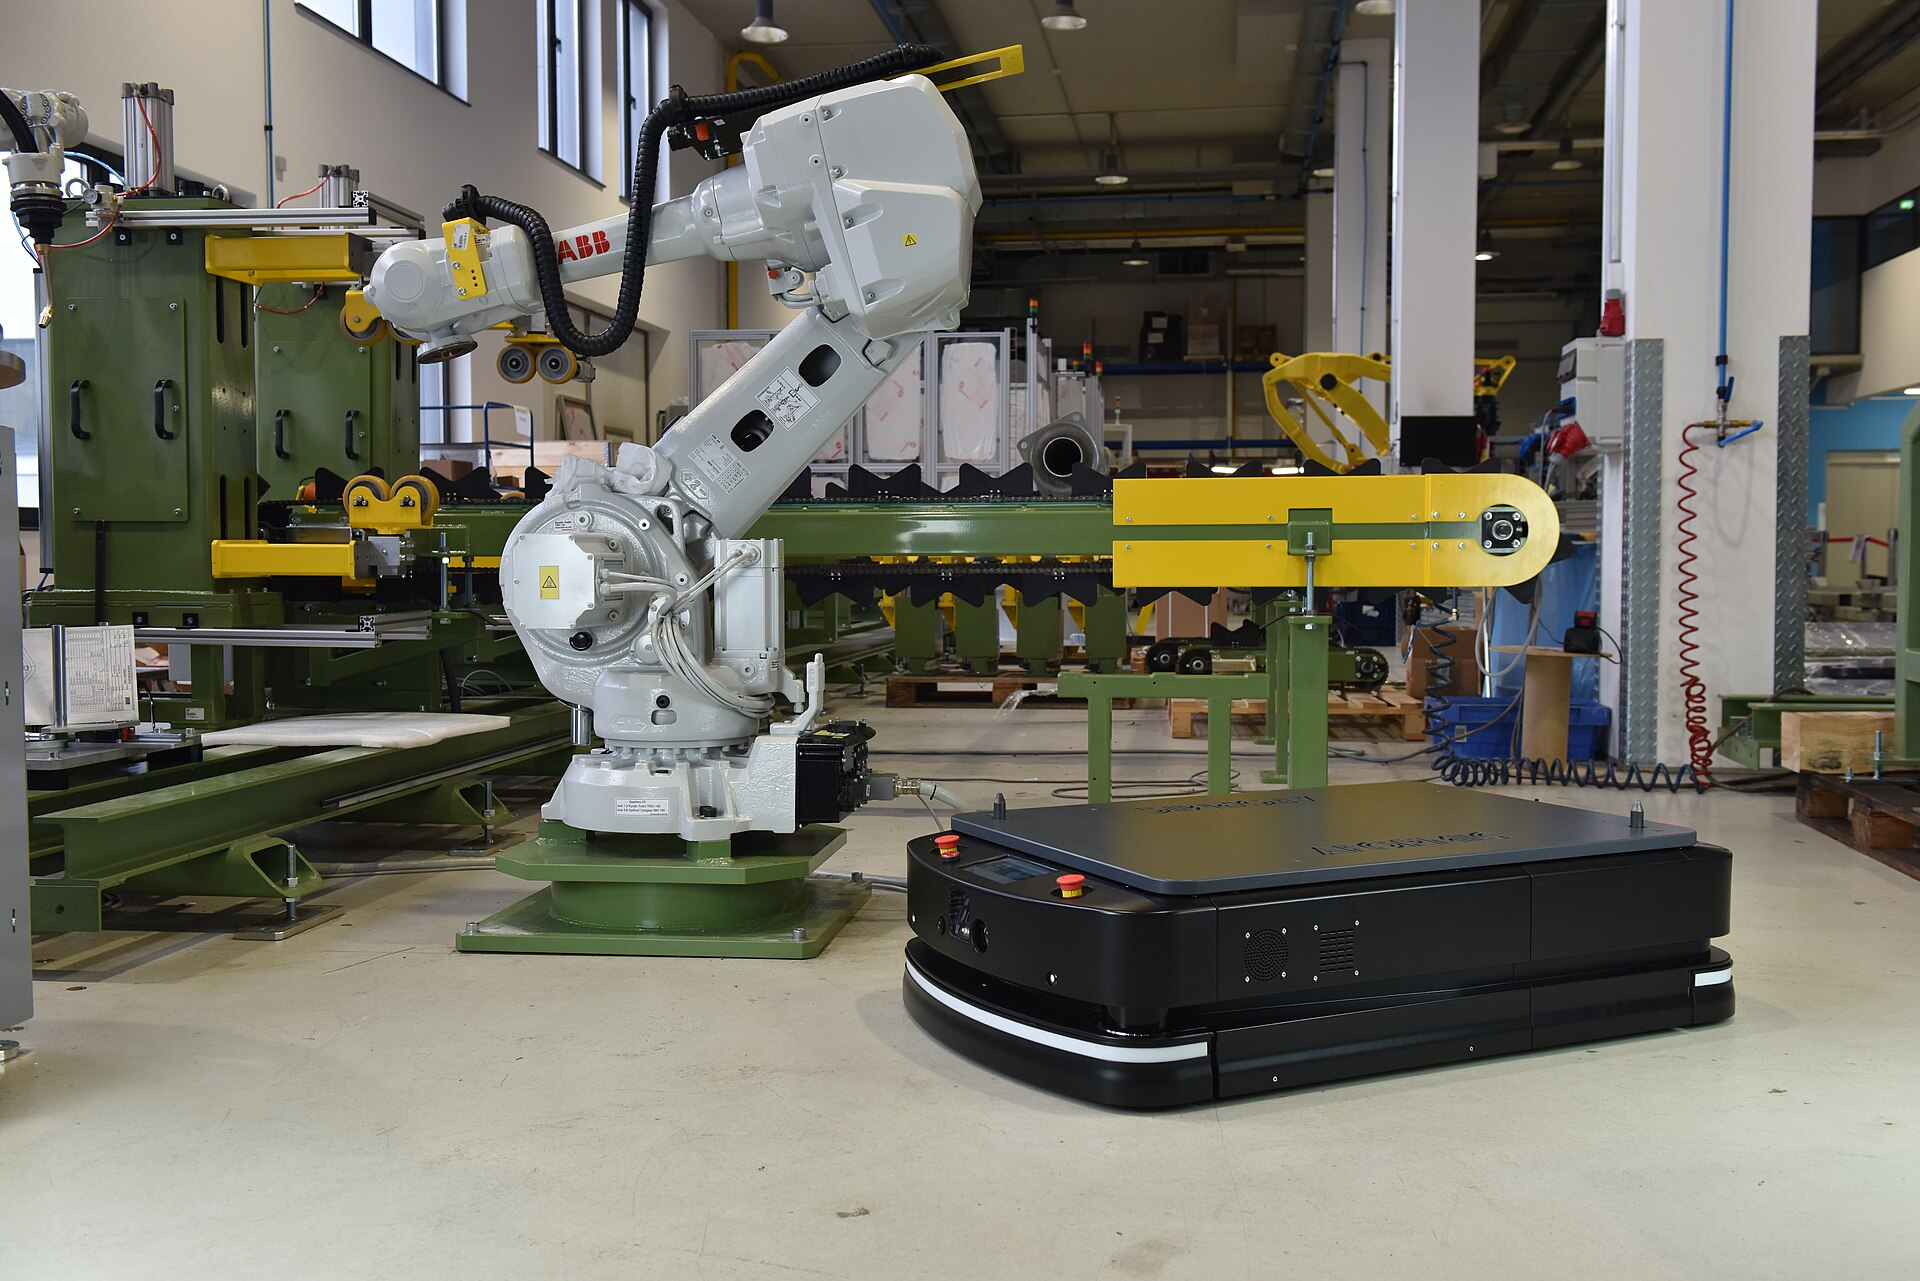
\includegraphics[width=\linewidth,height=3.6cm,keepaspectratio]{../../figures/r24_agv.jpg}\\
\credit{Industrial robot and AGV, Marta Veverica, CC BY-SA 4.0, via Wikimedia Commons}
\column{.56\textwidth}
\small
\renewcommand{\arraystretch}{1.15}
\begin{tabularx}{\linewidth}{@{}l X X@{}}
\toprule
 & \textbf{AGV} & \textbf{AMR}\\
\midrule
Guidance & wire, magnetic tape, QR floor codes & natural features (LiDAR map)\\
Obstacle & stops and waits & plans a path around it\\
Layout change & re-lay the tape & edit the map\\
Typical use & fixed, heavy, repetitive routes & changing routes, shared spaces\\
\bottomrule
\end{tabularx}

\vspace{1mm}
\begin{itemize}\small
\item \term{AGV}: automated guided vehicle (a train on invisible rails).
\item \term{AMR}: autonomous mobile robot (a taxi that finds its own way).
\end{itemize}
\end{columns}
\gofurther{AMRs localise with SLAM (simultaneous localisation and mapping) and drive with differential-drive kinematics (4.7).}
\end{frame}

% ---------------------------------------------------------------------
\begin{frame}{Worked example: how many AMRs do we need?}
\begin{columns}[T]
\column{.45\textwidth}
\centering
\begin{tikzpicture}[font=\scriptsize]
  \node[blk,minimum width=17mm,minimum height=10mm] (w) at (0,0) {warehouse\\(load)};
  \node[blk,minimum width=17mm,minimum height=10mm,fill=mkCream,draw=mkOrange] (c) at (4.4,0) {robot cell\\(unload)};
  \draw[sig] ([yshift=2mm]w.east) -- ([yshift=2mm]c.west) node[midway,above]{\SI{200}{m} loaded};
  \draw[sig] ([yshift=-2mm]c.west) -- ([yshift=-2mm]w.east) node[midway,below]{\SI{200}{m} empty};
  \node[mkGray] at (2.2,-1.2) {speed \SI{1}{m/s}, \SI{60}{s} to load or unload};
  \fill[mkOrange] (1.6,.5) rectangle ++(.5,.25); \fill[mkNavy] (1.7,.47) circle (.05) (2.0,.47) circle (.05);
\end{tikzpicture}

\vspace{2mm}
\begin{notebox}
\small Rule of thumb: plan 15--25\,\% spare capacity for charging, traffic and peaks.
\end{notebox}
\column{.52\textwidth}
\begin{keybox}[Step by step]
\small
1.\ Demand: \hl{60 transports per hour}\\[.5mm]
2.\ Travel: $2\cdot200/1=\SI{400}{s}$; handling $2\cdot60=\SI{120}{s}$\\[.5mm]
3.\ Round trip $=\SI{520}{s}\approx\SI{8.7}{min}$ $\Rightarrow$ $60/8.7\approx6.9$ trips/h per AMR\\[.5mm]
4.\ $60/6.9\approx8.7$ $\Rightarrow$ 9 AMRs; with 80\,\% availability $9/0.8\approx11.3$ $\Rightarrow$ \hl{12 AMRs}
\end{keybox}
\begin{eqbox}
\vspace{-2mm}
\[ N_\text{AMR}=\frac{\text{demand [trips/h]}\cdot t_\text{round trip}\,[\text{h}]}{\text{availability}} \]
\vspace{-4mm}
\end{eqbox}
\end{columns}
\end{frame}

% ---------------------------------------------------------------------
\begin{frame}{Flexible manufacturing system (FMS) cell}
\begin{columns}[T]
\column{.55\textwidth}
\centering
\begin{tikzpicture}[font=\scriptsize]
  \draw[mkGray,dashed,rounded corners] (-.3,-.3) rectangle (6.6,3.5);
  \node[blk,minimum width=13mm] (m1) at (.6,2.8) {CNC 1};
  \node[blk,minimum width=13mm] (m2) at (2.6,2.8) {CNC 2};
  \node[blk,minimum width=13mm] (m3) at (4.6,2.8) {wash /\\measure};
  \node[blk,minimum width=13mm,fill=mkCream,draw=mkOrange] (ls) at (.6,.3) {load /\\unload};
  \node[blk,minimum width=13mm] (as) at (4.6,.3) {pallet\\store};
  \draw[mkOrange,very thick,rounded corners] (0,1.55) -- (6.2,1.55);
  \node[mkOrange,above] at (5.6,1.55) {AGV / rail};
  \fill[mkNavy] (2.4,1.45) rectangle ++(.5,.22);
  \foreach \n in {m1,m2,m3}{\draw[thick,mkNavy,-{Latex}] (\n.south) -- ++(0,-.55);}
  \foreach \n in {ls,as}{\draw[thick,mkNavy,-{Latex}] (\n.north) -- ++(0,.55);}
  \node[blk,fill=mkSky!40] (cc) at (2.6,.3) {cell\\computer};
  \draw[mkMid,dashed] (cc) -- (ls) (cc) -- (as);
\end{tikzpicture}
\column{.43\textwidth}
\begin{itemize}\small
\item \term{FMS}: several CNC machines + automated transport + a computer that schedules jobs.
\item Parts ride on \term{pallets} with fixtures; any machine can take any pallet.
\item Robots load machines; AGVs or rail carts move pallets.
\end{itemize}
\begin{keybox}[Bottleneck example]
\small Stations take 40, 60 and \SI{45}{s} per part. The \hl{slowest} sets the pace: one part per \SI{60}{s} $=$ 60 parts/h.
\end{keybox}
\end{columns}
\end{frame}

% ---------------------------------------------------------------------
\begin{frame}{Collaborative robots (cobots)}
\begin{columns}[T]
\column{.42\textwidth}
\centering
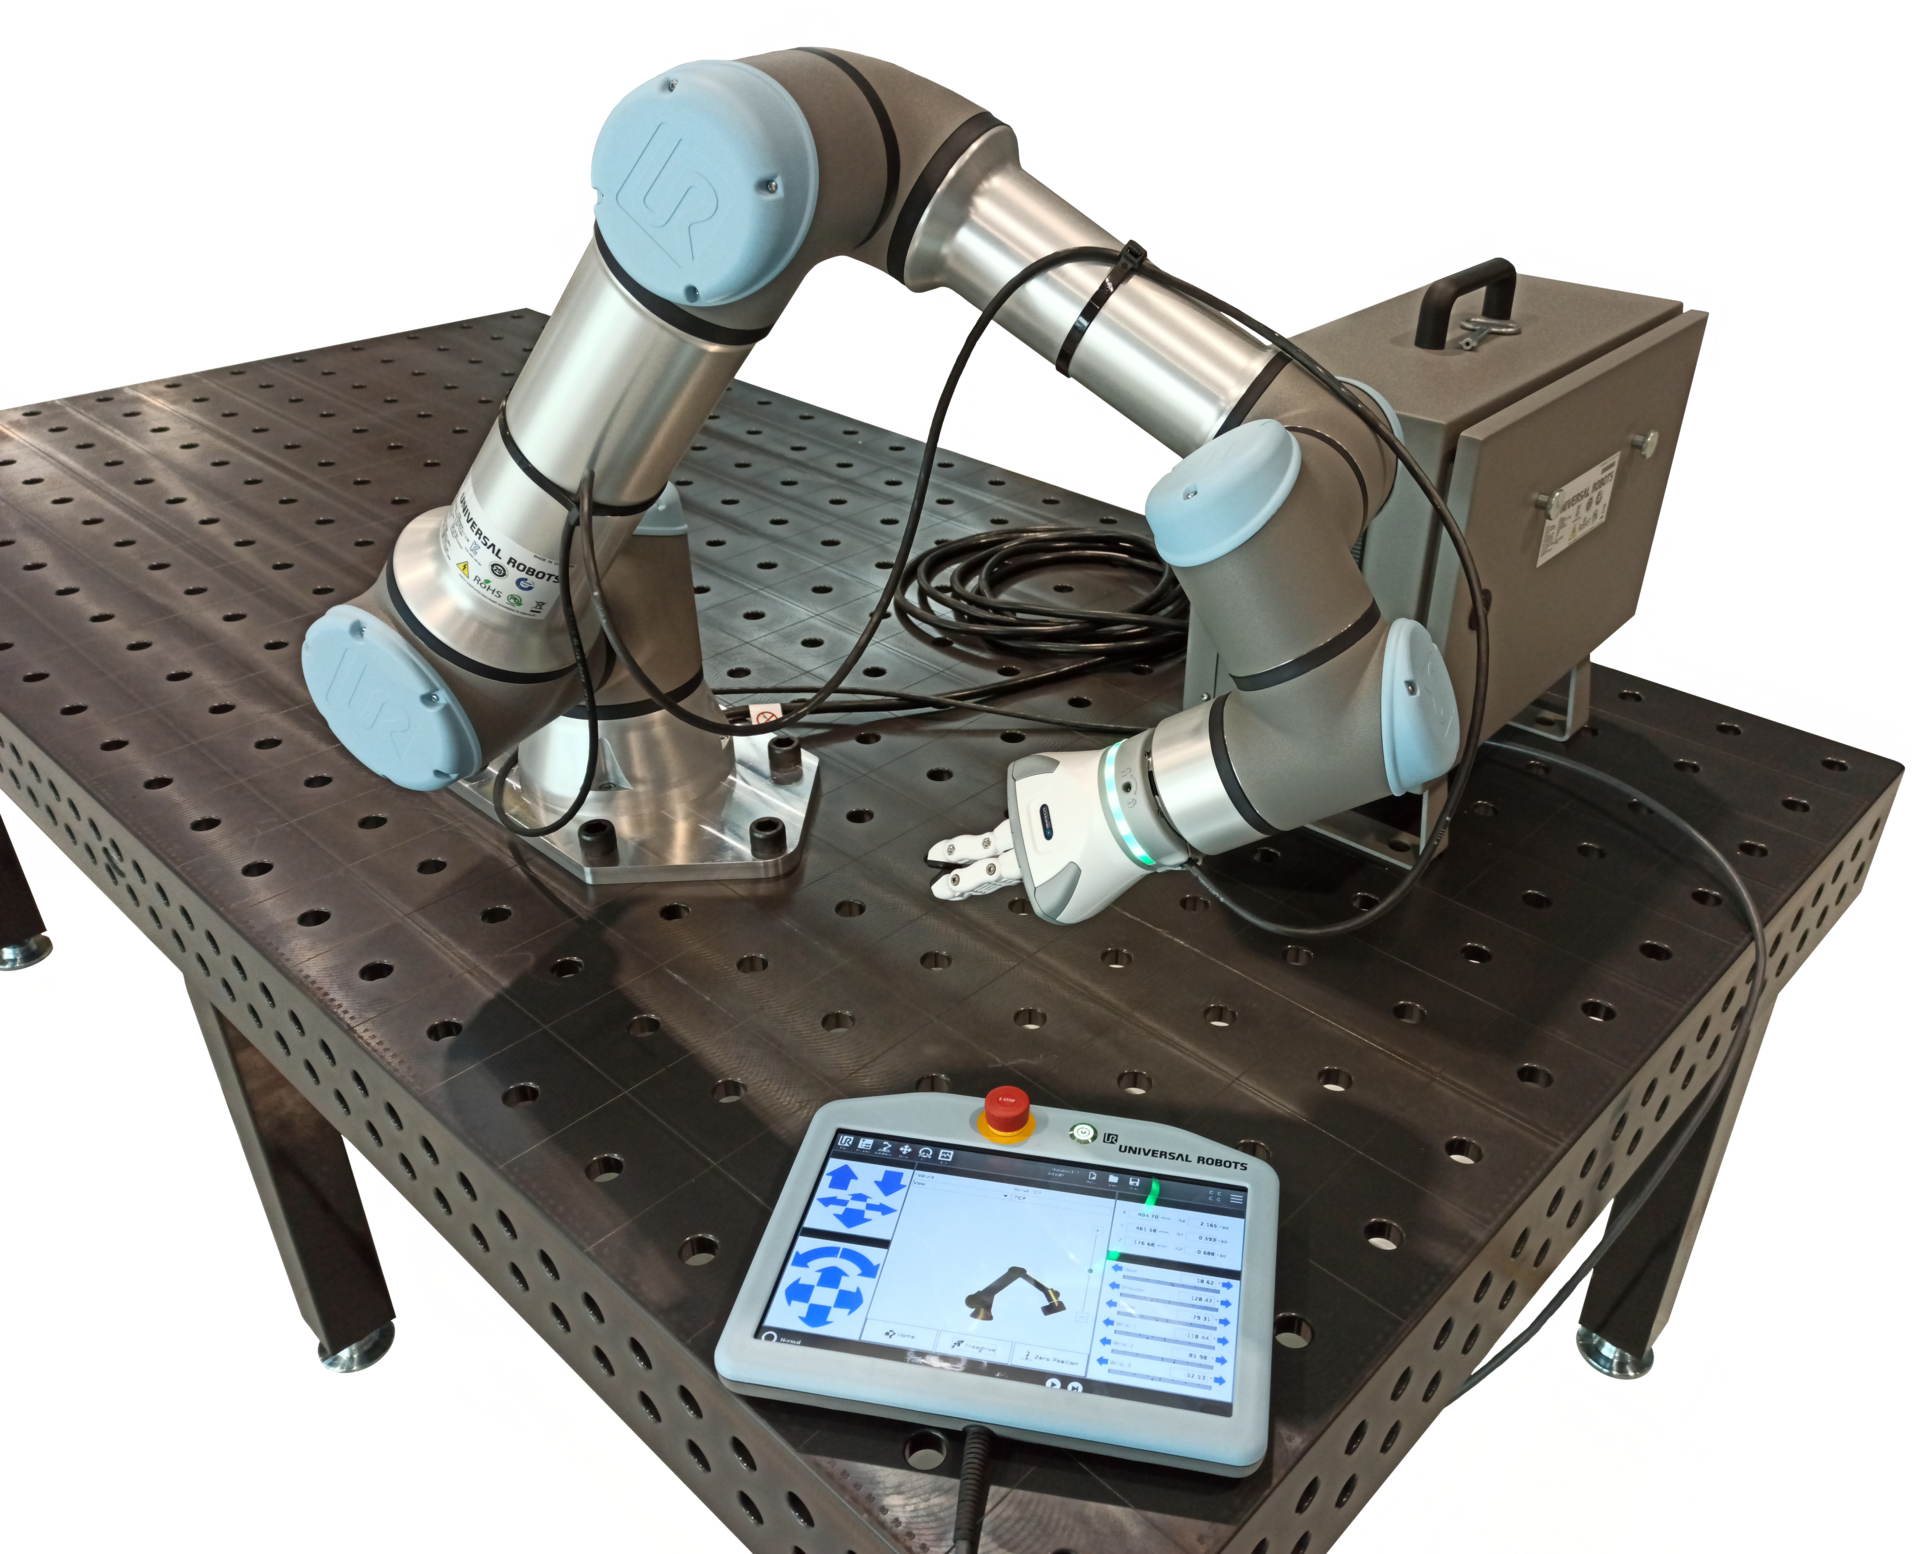
\includegraphics[width=\linewidth,height=4.0cm,keepaspectratio]{../../figures/r24_cobot.png}\\
\credit{UR16e robot arm, Auledas, CC BY-SA 4.0, via Wikimedia Commons}
\column{.56\textwidth}
\begin{defbox}[Definition]
\small A \term{cobot} is a robot designed to work \emph{in the same space} as people, without a fence, when the risk assessment allows it.
\end{defbox}
\begin{itemize}\small
\item Light arms, rounded shapes, no pinch points.
\item Joint torque or current sensing detects a collision and stops.
\item Speed and force are limited by safety settings.
\item Easy to teach by hand (hand guiding).
\end{itemize}
\begin{notebox}
\small A cobot with a knife in its gripper is \hl{not} safe. The \emph{application} is collaborative, not the robot alone.
\end{notebox}
\end{columns}
\end{frame}

% ---------------------------------------------------------------------
\begin{frame}{Human--robot collaboration: four modes}
\centering
\begin{tikzpicture}[font=\scriptsize]
  \foreach \i/\t/\s in {0/{Safety-rated\\monitored stop}/{robot stops while the\\person is in the shared space},
                         1/{Hand guiding}/{person moves the robot\\with an enabling handle},
                         2/{Speed \& separation\\monitoring}/{robot slows or stops as\\the person comes closer},
                         3/{Power \& force\\limiting}/{contact allowed, but forces\\stay below body limits}}{
    \begin{scope}[xshift=\i*3.7cm]
      \draw[mkBlue,thick,fill=mkLight,rounded corners] (0,0) rectangle (3.4,2.6);
      \node[font=\scriptsize\bfseries,align=center,text=mkBlue] at (1.7,2.25) {\t};
      \node[align=center,text=mkGray,font=\tiny] at (1.7,-.45) {\s};
      % robot base
      \fill[mkBlue] (.4,.3) rectangle (.9,.45);
      % person
      \fill[mkOrange] (2.7,1.25) circle (.13); \draw[mkOrange,line width=2pt] (2.7,1.1) -- (2.7,.6) (2.7,.6) -- (2.55,.3) (2.7,.6) -- (2.85,.3) (2.7,1.0) -- (2.45,.85);
    \end{scope}}
  % mode-specific arms
  \draw[mkBlue,line width=2.5pt] (.65,.45) -- (.9,1.3) -- (1.4,1.0); \node[mkRed,font=\bfseries] at (1.6,1.5) {STOP};
  \draw[mkBlue,line width=2.5pt] (4.35,.45) -- (4.7,1.3) -- (5.9,.95); \draw[mkOrange,line width=1.5pt] (6.15,.85) -- (5.95,.95);
  \draw[mkBlue,line width=2.5pt] (8.05,.45) -- (8.4,1.3) -- (8.9,1.0);
  \begin{scope}\clip (7.4,0) rectangle (10.8,2.0); \draw[mkSky,dashed] (8.2,.45) circle (1.0); \draw[mkOrange,dashed] (8.2,.45) circle (1.45);\end{scope}
  \draw[mkBlue,line width=2.5pt] (11.75,.45) -- (12.1,1.3) -- (13.2,1.05);
  \draw[mkRed,thick] (13.35,1.05) circle (.12); \node[mkRed,font=\tiny] at (13.0,1.6) {$F\le F_\text{max}$};
\end{tikzpicture}

\vspace{6mm}
\begin{columns}[T]
\column{.55\textwidth}
\begin{itemize}\small
\item Defined in \term{ISO 10218} (robots \& robot systems); \term{ISO/TS 15066} gives body-region force and pressure limits for contact.
\item Most real cells combine modes, e.g.\ speed \& separation plus a monitored stop.
\end{itemize}
\column{.42\textwidth}
\gofurther{in power \& force limiting, the energy of a contact $\tfrac12\mu v^2$ must stay below what the body region can absorb, $F_\text{max}^2/(2k)$, which caps the relative speed: $v_\text{max}=F_\text{max}/\sqrt{\mu k}$.}
\end{columns}
\end{frame}

% ---------------------------------------------------------------------
\begin{frame}{Check your understanding: material handling}
\begin{keybox}[Check your understanding]
\large
\begin{enumerate}
\item A conveyor drum of \SI{0.2}{m} diameter turns at \SI{0.5}{rev/s}. What is the belt speed?
\item An AGV meets a box left in the aisle. What does it do, and what would an AMR do?
\item A cobot carries a sharp deburring tool. Can the cell run without any safeguards? Why?
\end{enumerate}
\end{keybox}
\end{frame}

% ---------------------------------------------------------------------
\begin{frame}{Summary and key terms: material handling}
\begin{columns}[T]
\column{.52\textwidth}
\begin{itemize}\small
\item Parts spend most time waiting: flow matters as much as speed.
\item Conveyor speed $v=\pi D n/i$; tracking uses a belt encoder.
\item AGVs follow fixed guides; AMRs navigate with a map.
\item FMS: machines + transport + scheduling computer.
\item Cobots: four collaborative modes, judged per application.
\end{itemize}
\column{.45\textwidth}
\begin{defbox}[Key terms]
\small
\term{accumulation} parts queue on the belt\\
\term{conveyor tracking} robot follows the belt\\
\term{AGV / AMR} guided / autonomous vehicle\\
\term{FMS} flexible manufacturing system\\
\term{bottleneck} slowest station\\
\term{HRC} human--robot collaboration
\end{defbox}
{\scriptsize\color{mkGray} [Groover, 2019]; ISO 10218-2; ISO/TS 15066.}
\end{columns}
\end{frame}

% =====================================================================
\section{5.7 Safety and standards}

\begin{frame}{Why robots are dangerous}
\begin{columns}[T]
\column{.5\textwidth}
\centering
\begin{tikzpicture}
\begin{axis}[mkplot,width=\linewidth,height=4.3cm,xmin=0,xmax=3,ymin=0,ymax=100,
  xlabel={speed $v$ [m/s]},ylabel={kinetic energy $E$ [J]},legend pos=north west]
\addplot[mkBlue,thick,domain=0:3,samples=40] {0.5*5*x^2};
\addplot[mkOrange,thick,domain=0:3,samples=40] {0.5*20*x^2};
\legend{moving mass \SI{5}{kg}, moving mass \SI{20}{kg}}
\addplot[mark=*,mkOrange,only marks] coordinates {(2,40)};
\node[font=\tiny,anchor=west] at (axis cs:2.05,38) {\SI{40}{J}};
\end{axis}
\end{tikzpicture}
\column{.47\textwidth}
\begin{itemize}\small
\item Hazards: \term{impact}, \term{crushing} and \term{trapping}, flying parts, the tool itself (laser, weld arc, blade).
\item Robots move \emph{fast}, \emph{without warning} and may start unexpectedly.
\end{itemize}
\begin{eqbox}
\vspace{-2mm}
\[ E=\tfrac12\,m\,v^2 \]
\vspace{-4mm}
\end{eqbox}
\begin{keybox}[Worked example]
\small
1.\ Effective moving mass \SI{20}{kg} at \SI{2}{m/s}\\
2.\ $E=0.5\cdot20\cdot2^2=\SI{40}{J}$\\
3.\ Like a \SI{4}{kg} brick dropped from \SI{1}{m}: enough to break bones.
\end{keybox}
\end{columns}
\end{frame}

% ---------------------------------------------------------------------
\begin{frame}{ISO 12100: the risk assessment loop}
\begin{columns}[T]
\column{.55\textwidth}
\centering
\begin{tikzpicture}[font=\scriptsize,node distance=2.5mm,
  st/.style={draw=mkBlue,fill=mkPale,thick,rounded corners=2pt,minimum width=4.2cm,minimum height=5.5mm,align=center}]
  \node[st] (a) {1.\ Determine the limits of the machine};
  \node[st,below=of a] (b) {2.\ Identify hazards};
  \node[st,below=of b] (c) {3.\ Estimate risk (severity, probability)};
  \node[st,below=of c] (d) {4.\ Evaluate: is the risk acceptable?};
  \node[st,below=7mm of d,fill=mkCream,draw=mkOrange] (e) {5.\ Reduce risk (three-step method)};
  \node[st,right=6mm of d,minimum width=1.4cm,fill=mkGreen!20,draw=mkGreen] (ok) {done:\\document};
  \draw[sig] (a) -- (b); \draw[sig] (b) -- (c); \draw[sig] (c) -- (d);
  \draw[sig] (d) -- node[right]{no} (e);
  \draw[sig] (d) -- node[above]{yes} (ok);
  \draw[sig] (e.west) -- ++(-.4,0) |- (b.west);
  \draw[decorate,decoration={brace,amplitude=4pt,mirror},mkGray] ([xshift=-7mm]a.north west) -- ([xshift=-7mm]c.south west) node[midway,left=2mm,align=right]{risk\\analysis};
\end{tikzpicture}
\column{.43\textwidth}
\begin{defbox}[Definition]
\small \term{Risk} $=$ combination of the \hl{severity} of a possible harm and the \hl{probability} that it occurs.
\end{defbox}
\begin{itemize}\small
\item ISO 12100 is the basic (type A) standard for \emph{all} machinery.
\item It is a loop: after each safeguard, check again for new hazards.
\item The result is written down: the risk assessment file.
\end{itemize}
\end{columns}
\end{frame}

% ---------------------------------------------------------------------
\begin{frame}{Three-step risk reduction and the standards family}
\begin{columns}[T]
\column{.48\textwidth}
\centering
\begin{tikzpicture}[font=\scriptsize]
  \fill[mkBlue] (0,0) -- (5,0) -- (4.2,1.1) -- (.8,1.1) -- cycle;
  \fill[mkMid] (.8,1.15) -- (4.2,1.15) -- (3.4,2.25) -- (1.6,2.25) -- cycle;
  \fill[mkSky] (1.6,2.3) -- (3.4,2.3) -- (2.5,3.4) -- cycle;
  \node[white,align=center] at (2.5,.55) {\textbf{1.\ Inherently safe design}\\less speed, mass, force};
  \node[white,align=center] at (2.5,1.7) {\textbf{2.\ Safeguards}\\fences, curtains};
  \node[mkNavy,align=center] at (2.5,2.75) {\textbf{3.}\\info};
  \draw[sig,mkOrange] (5.4,.2) -- (5.4,3.2) node[midway,right,align=left,text=mkOrange]{less\\effective};
\end{tikzpicture}\\
{\scriptsize\color{mkGray} Step 3 $=$ warnings, signs, training, PPE.}
\column{.5\textwidth}
\centering
\begin{tikzpicture}[font=\scriptsize,node distance=2mm,
  sd/.style={draw=mkBlue,fill=mkPale,thick,rounded corners=2pt,text width=4.6cm,align=left,minimum height=6mm}]
  \node[sd] (A) {\textbf{Type A} \ ISO 12100: risk assessment};
  \node[sd,below=of A] (B) {\textbf{Type B} \ ISO 13849, IEC 62061 (safety controls); ISO 13855 (distances)};
  \node[sd,below=of B,fill=mkCream,draw=mkOrange] (C) {\textbf{Type C} \ ISO 10218-1/-2 (industrial robots); ISO/TS 15066 (collaboration)};
  \draw[sig] (A) -- (B); \draw[sig] (B) -- (C);
\end{tikzpicture}

\vspace{2mm}
\begin{itemize}\small
\item A: general, B: generic safety aspects, C: one machine type.
\item A type C standard takes priority for its machine.
\end{itemize}
\end{columns}
\end{frame}

% ---------------------------------------------------------------------
\begin{frame}{How strong must a safety function be? The risk graph}
\begin{columns}[T]
\column{.58\textwidth}
\centering
\begin{tikzpicture}[font=\scriptsize,xscale=1.05]
  \node[circle,fill=mkBlue,text=white,inner sep=1.5pt] (s) at (0,0) {start};
  \foreach \sy/\sl in {1.6/S1,-1.6/S2}{
    \draw[thick,mkNavy] (s) -- (1.1,\sy) node[midway,above,sloped,font=\tiny]{\sl};
    \foreach \fy/\fl in {.8/F1,-.8/F2}{
      \draw[thick,mkNavy] (1.1,\sy) -- (2.3,\sy+\fy*.5) node[midway,above,sloped,font=\tiny]{\fl};
      \foreach \py/\pl in {.2/P1,-.2/P2}{
        \draw[thick,mkNavy] (2.3,\sy+\fy*.5) -- (3.5,\sy+\fy*.5+\py) node[pos=.75,above,font=\tiny]{\pl};
      }}}
  \foreach \y/\p/\c in {2.2/a/mkGreen,1.8/b/mkGreen,1.4/b/mkGreen,1.0/c/mkAmber,-1.0/c/mkAmber,-1.4/d/mkOrange,-1.8/d/mkOrange,-2.2/e/mkRed}{
    \node[draw=\c,fill=\c!25,font=\tiny\bfseries,minimum width=5mm,inner sep=1pt] at (3.85,\y) {\p};}
  \node[font=\scriptsize\bfseries,text=mkBlue] at (3.85,2.65) {PL$_\text{r}$};
\end{tikzpicture}
\column{.4\textwidth}
\small
\begin{tabular}{@{}l l@{}}
\toprule
S & severity: S1 slight, S2 serious\\
F & exposure: F1 rare, F2 frequent\\
P & avoidance: P1 possible, P2 hardly\\
\bottomrule
\end{tabular}

\vspace{2mm}
\begin{itemize}\small
\item Result: the \term{required performance level} PL$_\text{r}$, from a (weak) to e (strong).
\item Robot safety functions are typically required at \hl{PL d}.
\end{itemize}
\begin{keybox}[Example]
\small Operator reaches into a robot cell several times per hour (F2), injury could be serious (S2), robot is fast (P2) $\Rightarrow$ \hl{PL e}.
\end{keybox}
\end{columns}
\end{frame}

% ---------------------------------------------------------------------
\begin{frame}{Performance level and redundant (two-channel) design}
\begin{columns}[T]
\column{.5\textwidth}
\centering
\begin{tikzpicture}[font=\scriptsize]
  \node[blk] (i1) at (0,1) {sensor\\ch.\ 1};
  \node[blk] (i2) at (0,-.2) {sensor\\ch.\ 2};
  \node[blk,fill=mkCream,draw=mkOrange] (l1) at (2.2,1) {logic 1};
  \node[blk,fill=mkCream,draw=mkOrange] (l2) at (2.2,-.2) {logic 2};
  \node[blk] (o1) at (4.4,1) {contactor\\K1};
  \node[blk] (o2) at (4.4,-.2) {contactor\\K2};
  \draw[sig] (i1) -- (l1); \draw[sig] (i2) -- (l2); \draw[sig] (l1) -- (o1); \draw[sig] (l2) -- (o2);
  \draw[mkRed,thick,{Latex}-{Latex},dashed] (l1) -- (l2) node[midway,right,font=\tiny]{cross-check};
  \draw[mkMid,thick,-{Latex}] (o2.south) -- ++(0,-.4) -| node[pos=.25,below,font=\tiny]{feedback (detect welded contact)} (l2.south);
  \node[mkGray] at (2.2,1.8) {Category 3: one fault does not lose the safety function};
\end{tikzpicture}
\column{.48\textwidth}
\small
\renewcommand{\arraystretch}{1.1}
\begin{tabular}{@{}c l@{}}
\toprule
\textbf{PL} & \textbf{dangerous failures per hour}\\
\midrule
a & $10^{-5}$ to $10^{-4}$\\
b & $3\cdot10^{-6}$ to $10^{-5}$\\
c & $10^{-6}$ to $3\cdot10^{-6}$\\
d & $10^{-7}$ to $10^{-6}$\\
e & $10^{-8}$ to $10^{-7}$\\
\bottomrule
\end{tabular}

\vspace{1mm}
\begin{itemize}\small
\item PL d: at most one dangerous failure in about \hl{100 years} of operation ($10^{-6}$/h $\approx$ 1 per 114 years).
\item Reached by \term{redundancy} + \term{diagnostics} + reliable parts.
\end{itemize}
\gofurther{ISO 13849-1 combines category, MTTF$_\text{D}$, diagnostic coverage and common-cause failure.}
\end{columns}
\end{frame}

% ---------------------------------------------------------------------
\begin{frame}{Light curtains and the safety distance}
\begin{columns}[T]
\column{.45\textwidth}
\centering
\begin{tikzpicture}[font=\scriptsize]
  \fill[mkPale] (2.6,0) rectangle (5,3);
  \node[mkBlue,align=center] at (3.9,1.5) {hazard\\zone};
  \fill[mkBlue] (0,0) rectangle (.2,3); \fill[mkBlue] (1.6,0) rectangle (1.8,3);
  \foreach \y in {.2,.5,...,2.9}{\draw[mkOrange] (.2,\y) -- (1.6,\y);}
  \node[above,align=center] at (.9,3) {light curtain};
  \draw[{Latex}-{Latex},mkNavy,thick] (1.8,-.3) -- (2.6,-.3) node[midway,below]{$S$};
  \fill[mkOrange] (-.8,1.9) circle (.16); \draw[mkOrange,line width=2pt] (-.8,1.75) -- (-.8,.9) (-.8,.9) -- (-1,.2) (-.8,.9) -- (-.6,.2) (-.8,1.6) -- (-.1,1.5);
\end{tikzpicture}
\begin{itemize}\small
\item Beams of infrared light; any blocked beam $\Rightarrow$ stop signal.
\item \term{Detection capability} $d$: \SI{14}{mm} finger, \SI{30}{mm} hand.
\end{itemize}
\column{.53\textwidth}
\begin{eqbox}
\vspace{-2mm}
\[ S=K\cdot T+C \qquad\text{(ISO 13855)} \]
\vspace{-4mm}
\end{eqbox}
{\footnotesize $S$ min.\ distance [mm], $K$ approach speed (\SI{2000}{mm/s} for a hand), $T$ total stopping time [s], $C$ intrusion allowance $=8(d-14)$ [mm].}
\begin{keybox}[Worked example]
\small
1.\ Curtain \SI{20}{ms} $+$ robot stop \SI{180}{ms} $\Rightarrow$ $T=\SI{0.2}{s}$\\
2.\ $d=\SI{14}{mm}$ $\Rightarrow$ $C=8\cdot(14-14)=0$\\
3.\ $S=2000\cdot0.2+0=\SI{400}{mm}$
\end{keybox}
\begin{notebox}
\small A slower-stopping robot needs the curtain \hl{further away}: measure the real stopping time!
\end{notebox}
\end{columns}
\end{frame}

% ---------------------------------------------------------------------
\begin{frame}{Laser scanners and speed \& separation monitoring}
\begin{columns}[T]
\column{.5\textwidth}
\centering
\begin{tikzpicture}[font=\scriptsize]
  \fill[mkCream] (0,0) -- (3.2,0) arc (0:180:3.2) -- cycle;
  \fill[mkAmber!50] (0,0) -- (2.2,0) arc (0:180:2.2) -- cycle;
  \fill[mkRed!35] (0,0) -- (1.2,0) arc (0:180:1.2) -- cycle;
  \node at (0,2.75) {warning field: slow down};
  \node at (0,1.75) {protective field: stop};
  \node[white,font=\scriptsize\bfseries] at (0,.75) {robot reach};
  \fill[mkBlue] (-.25,0) rectangle (.25,.2);
  \draw[mkMid,thick] (-3.4,0) -- (3.4,0);
  \fill[mkNavy] (2.2,.0) rectangle ++(.25,.18); \node[below,font=\tiny] at (2.3,0) {scanner};
  \fill[mkOrange] (2.7,1.6) circle (.13); \draw[mkOrange,line width=2pt] (2.7,1.45) -- (2.7,.95);
\end{tikzpicture}
\column{.48\textwidth}
\begin{itemize}\small
\item A \term{safety laser scanner} measures distance by light time-of-flight in a fan (Session 6.3).
\item Configurable \term{fields}: warning $\Rightarrow$ reduced speed; protective $\Rightarrow$ stop.
\item \term{Speed \& separation monitoring}: the allowed robot speed depends on how far away the person is.
\end{itemize}
\begin{keybox}[Intuition]
\small Like a car's adaptive cruise control: the closer the car ahead, the slower you go, and you must always be able to stop in time.
\end{keybox}
\end{columns}
\end{frame}

% ---------------------------------------------------------------------
\begin{frame}{Emergency stop, stop categories and the safety PLC}
\begin{columns}[T]
\column{.5\textwidth}
\centering
\begin{tikzpicture}
\begin{axis}[mkplot,width=\linewidth,height=4.2cm,xmin=0,xmax=1,ymin=0,ymax=1.15,
  xlabel={time after stop request [s]},ylabel={speed (normalised)},legend pos=north east]
\addplot[mkBlue,thick,domain=0:1,samples=80] {exp(-x/0.25)};
\addplot[mkOrange,thick] coordinates {(0,1) (0.3,0) (1,0)};
\addplot[mkSky,thick,dashed] coordinates {(0,1) (0.3,0) (1,0)};
\legend{Cat.\ 0: power cut (coasts / brake), Cat.\ 1: braked by drive then power off, Cat.\ 2: braked; power stays on}
\end{axis}
\end{tikzpicture}
{\scriptsize\color{mkGray} Stop categories of IEC 60204-1 (illustration).}
\column{.48\textwidth}
\begin{itemize}\small
\item \term{E-stop}: red mushroom button on yellow; latching, two channels; usually Cat.\ 0 or 1.
\item \term{Safety PLC}: redundant processors, self-tests, certified for PL e; reads curtains, door switches, scanners.
\item \term{Safe torque off (STO)}: the drive removes torque without opening the motor cable.
\end{itemize}
\begin{notebox}
\small Standard PLC: run the process. Safety PLC: decide whether the process may run at all.
\end{notebox}
\end{columns}
\end{frame}

% ---------------------------------------------------------------------
\begin{frame}{Check your understanding: safety}
\begin{keybox}[Check your understanding]
\large
\begin{enumerate}
\item List the three steps of ISO 12100 risk reduction in order of preference.
\item A light curtain sees \SI{14}{mm} objects; total stopping time is \SI{0.15}{s}. What is the minimum safety distance?
\item Why does a safety function use two channels instead of one very good channel?
\end{enumerate}
\end{keybox}
\end{frame}

% ---------------------------------------------------------------------
\begin{frame}{Summary and key terms: safety and standards}
\begin{columns}[T]
\column{.52\textwidth}
\begin{itemize}\small
\item ISO 12100: limits $\rightarrow$ hazards $\rightarrow$ estimate $\rightarrow$ evaluate $\rightarrow$ reduce, repeat.
\item Prefer safe design, then safeguards, then information.
\item Risk graph gives PL$_\text{r}$; redundancy + diagnostics reach it.
\item Safety distance $S=KT+C$; stopping time matters.
\item Robot standards: ISO 10218, ISO/TS 15066.
\end{itemize}
\column{.45\textwidth}
\begin{defbox}[Key terms]
\small
\term{risk} severity $\times$ probability of harm\\
\term{PL} performance level a--e\\
\term{category} structure (e.g.\ two channels)\\
\term{safeguard} guard or protective device\\
\term{STO} safe torque off\\
\term{protective field} zone that triggers a stop
\end{defbox}
{\scriptsize\color{mkGray} ISO 12100; ISO 13849-1; ISO 13855; IEC 60204-1.}
\end{columns}
\end{frame}

% =====================================================================
\section{6.1 Sensors and measurement principles}

\begin{frame}{The senses of a robot cell}
\begin{columns}[T]
\column{.55\textwidth}
\centering
\begin{tikzpicture}[font=\scriptsize,scale=.9]
  \fill[mkBlue] (0,0) rectangle (1,.25);
  \draw[mkBlue,line width=5pt,line cap=round] (.5,.25) -- (.9,1.9) -- (2.5,2.3);
  \fill[mkOrange] (.9,1.9) circle (.13) (.5,.3) circle (.13);
  \draw[mkNavy,thick,fill=mkCream] (2.5,2.15) rectangle (2.75,2.45);
  \draw[mkNavy,thick] (2.75,2.2) -- (3.0,2.05) (2.75,2.4) -- (3.0,2.55);
  \fill[mkPale] (1.8,.0) rectangle (4.5,.4); \draw[fill=mkOrange] (2.8,.4) rectangle ++(.4,.3);
  \draw[mkSky,fill=mkSky!40] (3.2,3.3) rectangle ++(.4,.25); \draw[mkSky,dashed] (3.4,3.3) -- (2.7,.7) (3.4,3.3) -- (3.6,.7);
  \foreach \y in {.2,.6,...,2.6}{\draw[mkOrange,thin] (-1.6,\y) -- (-1.1,\y);}
  \node[align=left,anchor=west] at (-2.6,3.1) (enc) {\hl{encoders} in every joint};
  \draw[mkGray] (enc.south) -- (.85,1.95);
  \node[align=left,anchor=west] at (3.7,2.5) {\hl{F/T sensor}\\at the wrist};
  \node[align=left,anchor=west] at (3.7,3.4) {\hl{camera}};
  \node[align=left,anchor=west] at (4.6,.25) {\hl{proximity}\\on conveyor};
  \node[align=center] at (-1.35,-.3) {\hl{light curtain}};
\end{tikzpicture}
\column{.43\textwidth}
\begin{itemize}\small
\item \term{Proprioceptive}: the robot senses \emph{itself} (joint angles, motor current).
\item \term{Exteroceptive}: senses the \emph{world} (parts, people, forces).
\item A typical cell has dozens of sensors; each one is an input to a controller or a PLC.
\end{itemize}
\begin{keybox}[Analogy]
\small Close your eyes and touch your nose: that is proprioception. Seeing the cup you reach for is exteroception.
\end{keybox}
\end{columns}
\end{frame}

% ---------------------------------------------------------------------
\begin{frame}{The measurement chain}
\centering
\begin{tikzpicture}[font=\scriptsize,node distance=12mm,scale=.8,transform shape]
  \node[blk,fill=mkCream,draw=mkOrange] (q) {measurand\\(force, angle, \dots)};
  \node[blk,right=of q] (s) {sensor /\\transducer};
  \node[blk,right=of s] (c) {signal\\conditioning};
  \node[blk,right=of c] (a) {ADC /\\counter};
  \node[blk,right=of a] (p) {processing\\(scale, filter)};
  \node[blk,right=of p,fill=mkSky!40] (u) {controller\\or PLC};
  \draw[sig] (q) -- (s); \draw[sig] (s) -- node[above,lbl]{mV, $\Delta R$} (c); \draw[sig] (c) -- node[above,lbl]{0--10 V} (a);
  \draw[sig] (a) -- node[above,lbl]{bits} (p); \draw[sig] (p) -- node[above,lbl]{N, rad} (u);
  \foreach \n in {s,c,a,p}{\draw[mkRed,-{Latex},thin] ($(\n.south)+(0,-.55)$) -- (\n.south);}
  \node[mkRed,font=\tiny] at ($(c.south)!.5!(a.south)+(0,-.75)$) {each stage adds error, noise and delay};
\end{tikzpicture}

\vspace{5mm}
\begin{columns}[T]
\column{.5\textwidth}
\begin{itemize}\small
\item \term{Transducer}: converts one physical quantity into another (strain $\rightarrow$ resistance).
\item \term{Signal conditioning}: amplify, filter, isolate, linearise.
\end{itemize}
\column{.47\textwidth}
\begin{notebox}
\small The chain is only as good as its weakest link: a perfect sensor with a noisy cable gives a noisy measurement. Sampling and filtering come on W2D5 (6.5, 6.6).
\end{notebox}
\end{columns}
\end{frame}

% ---------------------------------------------------------------------
\begin{frame}{Static characteristic: sensitivity, offset, range, linearity}
\begin{columns}[T]
\column{.52\textwidth}
\centering
\begin{tikzpicture}
\begin{axis}[mkplot,width=\linewidth,height=4.6cm,xmin=0,xmax=10,ymin=0,ymax=2.8,
  xlabel={input $x$ (e.g.\ force [N])},ylabel={output $y$ [V]},legend pos=north west]
\addplot[mkSky,thick,dashed,domain=0:10] {0.4+0.2*x};
\addplot[mkBlue,thick,domain=0:10,samples=60] {0.4+0.2*x+0.12*sin(deg(x*pi/10))};
\legend{ideal straight line, real sensor}
\draw[mkOrange,{Latex}-{Latex},thick] (axis cs:5,1.4) -- (axis cs:5,1.52);
\node[font=\tiny,anchor=west,text=mkOrange] at (axis cs:5.2,1.35) {max.\ deviation};
\node[font=\tiny,anchor=west] at (axis cs:.2,.25) {offset \SI{0.4}{V}};
\draw[mkMid,thick] (axis cs:7,1.8) -- (axis cs:8,1.8) -- (axis cs:8,2.0);
\node[font=\tiny,anchor=north] at (axis cs:7.8,1.78) {slope $=$ sensitivity};
\end{axis}
\end{tikzpicture}
\column{.46\textwidth}
\begin{eqbox}
\vspace{-2mm}
\[ y=y_0+S\,x \]
\vspace{-4mm}
\end{eqbox}
{\footnotesize $S$ \term{sensitivity} [V/N], $y_0$ \term{offset} [V].}
\begin{itemize}\small
\item \term{Range}: smallest to largest input, e.g.\ 0--\SI{10}{N}; \term{full scale} (FS) $=\SI{10}{N}$.
\item \term{Linearity error}: largest gap to the straight line, in \% of FS.
\end{itemize}
\begin{keybox}[Example]
\small Max.\ gap $\SI{0.12}{V}$ on an output span of $\SI{2.0}{V}$ $\Rightarrow$ linearity error $0.12/2.0=6\,\%$ FS.
\end{keybox}
\end{columns}
\end{frame}

% ---------------------------------------------------------------------
\begin{frame}{Accuracy, precision and resolution}
\begin{columns}[T]
\column{.5\textwidth}
\centering
\begin{tikzpicture}[font=\scriptsize,scale=.92]
  \foreach \cx/\cy/\t/\px/\py/\spr in {0/0/{accurate \& precise}/0/0/.12, 2.5/0/{precise, not accurate}/.45/.35/.12, 0/-2.5/{accurate, not precise}/0/0/.5, 2.5/-2.5/{neither}/.4/-.3/.5}{
    \begin{scope}[shift={(\cx,\cy)}]
      \fill[mkPale] (0,0) circle (1); \draw[mkSky] (0,0) circle (.66); \draw[mkSky] (0,0) circle (.33);
      \fill[mkOrange] (0,0) circle (.06);
      \foreach \a/\r in {10/1,80/.8,150/1,220/.7,290/.9,340/.6}{
        \fill[mkBlue] ({\px+\spr*\r*cos(\a)},{\py+\spr*\r*sin(\a)}) circle (.055);}
      \node[below] at (0,-1) {\t};
    \end{scope}}
\end{tikzpicture}
\column{.48\textwidth}
\begin{defbox}[Refresher: the dartboard picture]
\small
\term{Accuracy}: how close the darts land to the bull's-eye (true value).\\
\term{Precision} (repeatability): how tightly they cluster.\\
\term{Resolution}: the smallest change the sensor can show.
\end{defbox}
\begin{keybox}[Robots too]
\small A typical industrial robot repeats a taught point to about \SI{\pm0.05}{mm} (precision) but reaches a \emph{computed} point only to a few tenths of a mm (accuracy) [ISO 9283].
\end{keybox}
\end{columns}
\end{frame}

% ---------------------------------------------------------------------
\begin{frame}{Random and systematic errors}
\begin{columns}[T]
\column{.5\textwidth}
\centering
\begin{tikzpicture}
\begin{axis}[mkplot,width=\linewidth,height=4.3cm,xmin=9.4,xmax=10.8,ymin=0,ymax=3,
  xlabel={reading [kg]},ylabel={how often},ytick=\empty]
\addplot[mkBlue,thick,fill=mkPale,domain=9.5:10.7,samples=80] {2.5*exp(-(x-10.1)^2/(2*0.16^2))} \closedcycle;
\draw[mkOrange,thick] (axis cs:10.0,0) -- (axis cs:10.0,2.9);
\draw[mkBlue,dashed] (axis cs:10.1,0) -- (axis cs:10.1,2.6);
\node[font=\tiny,text=mkOrange,anchor=east] at (axis cs:9.98,2.7) {true 10.0};
\draw[{Latex}-{Latex},mkNavy] (axis cs:10.1,1.52) -- (axis cs:10.26,1.52) node[right,font=\tiny]{$\sigma$};
\node[font=\tiny,anchor=west] at (axis cs:10.12,2.75) {mean 10.1};
\end{axis}
\end{tikzpicture}
\begin{itemize}\small
\item \term{Systematic error} (bias): mean $-$ true; fixed by \hl{calibration}.
\item \term{Random error}: spread $\sigma$; reduced by \hl{averaging}.
\end{itemize}
\column{.48\textwidth}
\begin{eqbox}
\vspace{-2mm}
\[ \bar x=\tfrac1n\textstyle\sum x_i,\quad \sigma=\sqrt{\tfrac{1}{n-1}\textstyle\sum (x_i-\bar x)^2} \]
\vspace{-4mm}
\end{eqbox}
\begin{keybox}[Worked example: five readings]
\small
1.\ Readings: 10.2, 10.0, 10.1, 9.9, 10.3 kg\\
2.\ Mean $\bar x=50.5/5=\SI{10.1}{kg}$ $\Rightarrow$ bias $+\SI{0.1}{kg}$\\
3.\ Deviations: $0.1,-0.1,0,-0.2,0.2$; squares sum $0.10$\\
4.\ $\sigma=\sqrt{0.10/4}\approx\SI{0.16}{kg}$
\end{keybox}
\end{columns}
\end{frame}

% ---------------------------------------------------------------------
\begin{frame}{Calibration: making the numbers right}
\begin{columns}[T]
\column{.48\textwidth}
\centering
\begin{tikzpicture}
\begin{axis}[mkplot,width=\linewidth,height=4.4cm,xmin=0,xmax=11,ymin=0,ymax=2.8,
  xlabel={reference mass [kg]},ylabel={sensor output [V]}]
\addplot[mkBlue,thick,domain=0:11] {0.4+0.2*x};
\addplot[mkOrange,only marks,mark=*] coordinates {(0,0.4) (10,2.4)};
\addplot[mkMid,thick,dashed] coordinates {(0,1.3) (4.5,1.3) (4.5,0)};
\node[font=\tiny,anchor=south west] at (axis cs:0.2,0.45) {point 1};
\node[font=\tiny,anchor=north west] at (axis cs:10.1,2.35) {point 2};
\node[font=\tiny,anchor=south] at (axis cs:2.3,1.33) {reading \SI{1.30}{V}};
\end{axis}
\end{tikzpicture}
\column{.5\textwidth}
\begin{itemize}\small
\item Apply known inputs (\term{reference standards}), record outputs, fit a line.
\item Then invert the line to turn volts into kilograms.
\end{itemize}
\begin{keybox}[Worked example: two-point calibration]
\small
1.\ \SI{0}{kg} $\rightarrow$ \SI{0.40}{V}; \SI{10}{kg} $\rightarrow$ \SI{2.40}{V}\\
2.\ Sensitivity $S=(2.40-0.40)/10=\SI{0.20}{V/kg}$\\
3.\ Offset $y_0=\SI{0.40}{V}$\\
4.\ Reading \SI{1.30}{V}: $x=(1.30-0.40)/0.20=\SI{4.5}{kg}$
\end{keybox}
\gofurther{in robotics, ``calibration'' also means identifying the robot's true link lengths, camera parameters or tool frame (W2D5).}
\end{columns}
\end{frame}

% ---------------------------------------------------------------------
\begin{frame}{Dynamic behaviour: sensors are not instant}
\begin{columns}[T]
\column{.52\textwidth}
\centering
\begin{tikzpicture}
\begin{axis}[mkplot,width=\linewidth,height=4.4cm,xmin=0,xmax=5,ymin=0,ymax=1.15,
  xlabel={time $t/\tau$},ylabel={output / final value},legend pos=south east]
\addplot[mkSky,thick,dashed] coordinates {(0,0) (0,1) (5,1)};
\addplot[mkBlue,thick,domain=0:5,samples=80] {1-exp(-x)};
\addplot[mkOrange,only marks,mark=*] coordinates {(1,0.632) (3,0.95)};
\node[font=\tiny,anchor=west] at (axis cs:1.1,.6) {63\,\% at $t=\tau$};
\node[font=\tiny,anchor=north west] at (axis cs:3.05,.93) {95\,\% at $3\tau$};
\legend{true value (step), sensor reading}
\end{axis}
\end{tikzpicture}
\column{.46\textwidth}
\begin{defbox}[Analogy: a kitchen thermometer]
\small Put it in hot soup: the reading climbs for a while before it settles. The sensor needs time to ``catch up''.
\end{defbox}
\begin{eqbox}
\vspace{-2mm}
\[ y(t)=y_\infty\left(1-e^{-t/\tau}\right) \]
\vspace{-4mm}
\end{eqbox}
{\footnotesize $\tau$ \term{time constant} [s]. Same first-order response as W1D2 (2.2).}
\begin{keybox}[Example]
\small $\tau=\SI{2}{ms}$ $\Rightarrow$ 95\,\% after $3\tau=\SI{6}{ms}$; a \SI{1}{kHz} control loop sees the change only after six cycles.
\end{keybox}
\end{columns}
\end{frame}

% ---------------------------------------------------------------------
\begin{frame}{Check your understanding: measurement principles}
\begin{keybox}[Check your understanding]
\large
\begin{enumerate}
\item A scale shows 10.2, 10.2, 10.3\,kg for a true 10.0\,kg mass. Is it accurate, precise, both or neither?
\item A sensor reads \SI{1.0}{V} at \SI{0}{N} and \SI{3.0}{V} at \SI{100}{N}. What force gives \SI{2.2}{V}?
\item A temperature probe has $\tau=\SI{4}{s}$. How long until it shows 95\,\% of a sudden change?
\end{enumerate}
\end{keybox}
\end{frame}

% ---------------------------------------------------------------------
\begin{frame}{Summary and key terms: measurement principles}
\begin{columns}[T]
\column{.52\textwidth}
\begin{itemize}\small
\item Measurement chain: sensor $\rightarrow$ conditioning $\rightarrow$ ADC $\rightarrow$ processing.
\item Static: sensitivity, offset, range, linearity.
\item Accuracy $\neq$ precision $\neq$ resolution.
\item Bias $\rightarrow$ calibrate; noise $\rightarrow$ average.
\item Dynamic: time constant $\tau$, 95\,\% after $3\tau$.
\end{itemize}
\column{.45\textwidth}
\begin{defbox}[Key terms]
\small
\term{transducer} converts one quantity to another\\
\term{sensitivity} output change per input change\\
\term{full scale} largest rated input\\
\term{bias} systematic error\\
\term{repeatability} precision of repeated readings\\
\term{time constant} 63\,\% response time
\end{defbox}
{\scriptsize\color{mkGray} [Fraden, 2016]; [Bentley, 2005]; ISO 9283.}
\end{columns}
\end{frame}

% =====================================================================
\section{6.2 Position and motion sensors}

\begin{frame}{Where position sensors sit in a robot joint}
\begin{columns}[T]
\column{.55\textwidth}
\centering
\begin{tikzpicture}[font=\scriptsize]
  \draw[thick,mkNavy,fill=mkPale] (0,0) rectangle (1.6,1.2); \node at (.8,.6) {motor};
  \draw[thick,mkNavy,fill=mkSky!40] (-.6,.2) rectangle (0,1.0); \node[rotate=90] at (-.3,.6) {\tiny encoder};
  \draw[thick,mkNavy] (1.6,.6) -- (2.3,.6);
  \draw[thick,mkNavy,fill=mkCream] (2.3,.1) rectangle (3.5,1.1); \node[align=center] at (2.9,.6) {gear\\$i=100$};
  \draw[thick,mkNavy] (3.5,.6) -- (4.0,.6);
  \draw[thick,mkOrange,fill=mkSky!40] (4.0,.2) rectangle (4.4,1.0); \node[rotate=90] at (4.2,.6) {\tiny 2nd enc.};
  \draw[mkBlue,line width=4pt] (4.4,.6) -- (6.2,1.5);
  \node[mkGray,align=center] at (-.3,-.4) {motor side\\(standard)};
  \node[mkGray,align=center] at (4.2,-.4) {load side\\(optional)};
  \draw[mkRed,{Latex}-{Latex}] (2.3,1.4) -- (3.5,1.4) node[midway,above,font=\tiny]{backlash, elasticity};
\end{tikzpicture}

\vspace{2mm}
\begin{keybox}[Worked example: gear helps resolution]
\small
1.\ Motor encoder: $2^{17}=131\,072$ counts/rev\\
2.\ Gear $i=100$: $13.1$ million counts per joint rev\\
3.\ $360^\circ/13.1\cdot10^6\approx 0.00003^\circ$ per count
\end{keybox}
\column{.43\textwidth}
\begin{itemize}\small
\item Every robot joint has a sensor on the \hl{motor shaft}; the gear multiplies its resolution.
\item But the gear's backlash and twist are \emph{not} seen by a motor-side sensor.
\item High-accuracy robots add a \term{secondary (load-side) encoder}.
\end{itemize}
\begin{notebox}
\small Today: encoders, resolvers and inertial sensors (IMU). Cameras: W2D5 (6.4).
\end{notebox}
\end{columns}
\end{frame}

% ---------------------------------------------------------------------
\begin{frame}{Refresher: binary numbers and Gray code}
\begin{columns}[T]
\column{.5\textwidth}
\begin{defbox}[Refresher: binary]
\small
Each bit is a power of 2: $101_2=1\cdot4+0\cdot2+1\cdot1=5$.\\
$N$ bits give $2^N$ values: 3 bits $\rightarrow 8$, 12 bits $\rightarrow 4096$, 17 bits $\rightarrow 131\,072$.
\end{defbox}
\small
\renewcommand{\arraystretch}{1.05}
\centering
\begin{tabular}{@{}c c c@{}}
\toprule
\textbf{Value} & \textbf{Binary} & \textbf{Gray}\\
\midrule
2 & 010 & 011\\
3 & \hl{011} & 010\\
4 & \hl{100} & 110\\
5 & 101 & 111\\
\bottomrule
\end{tabular}
\column{.47\textwidth}
\centering
\begin{tikzpicture}[scale=.85]
  \foreach \k/\b/\c/\d in {0/0/0/0,1/0/0/1,2/0/1/1,3/0/1/0,4/1/1/0,5/1/1/1,6/1/0/1,7/1/0/0}{
    \pgfmathsetmacro{\aa}{90-\k*45}\pgfmathsetmacro{\ab}{90-(\k+1)*45}
    \ifnum\b=1 \fill[mkBlue] (\aa:.35) arc (\aa:\ab:.35) -- (\ab:.6) arc (\ab:\aa:.6) -- cycle; \fi
    \ifnum\c=1 \fill[mkMid] (\aa:.6) arc (\aa:\ab:.6) -- (\ab:.85) arc (\ab:\aa:.85) -- cycle; \fi
    \ifnum\d=1 \fill[mkOrange] (\aa:.85) arc (\aa:\ab:.85) -- (\ab:1.1) arc (\ab:\aa:1.1) -- cycle; \fi
    \draw[mkGray,very thin] (\aa:.35) -- (\aa:1.1);
    \pgfmathsetmacro{\am}{90-\k*45-22.5}
    \node[font=\tiny,mkNavy] at (\am:1.3) {\b\c\d};
  }
  \draw[mkGray] (0,0) circle (.35) circle (.6) circle (.85) circle (1.1);
\end{tikzpicture}\\
{\scriptsize 3-bit Gray-code disk}
\begin{itemize}\small
\item Binary $3\rightarrow4$: \hl{all 3 bits} flip; if they flip at slightly different moments the reader may see a wrong value.
\item \term{Gray code}: only \hl{one bit} changes per step $\Rightarrow$ no false readings.
\end{itemize}
\end{columns}
\end{frame}

% ---------------------------------------------------------------------
\begin{frame}{Optical incremental encoders}
\begin{columns}[T]
\column{.45\textwidth}
\centering
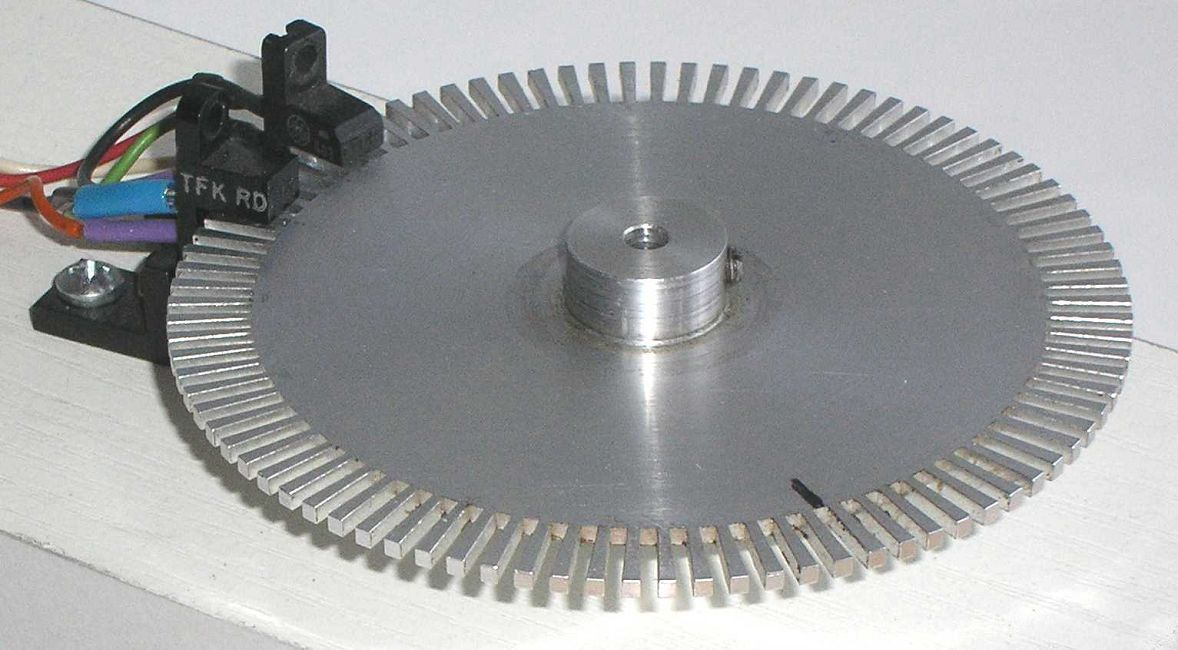
\includegraphics[width=\linewidth,height=4.2cm,keepaspectratio]{../../figures/d5_encoder_model.jpg}\\
\credit{Encoder model, Rrudzik, CC BY-SA 4.0, via Wikimedia Commons}
\column{.52\textwidth}
\begin{itemize}\small
\item An LED shines through a disk with $N$ slits (lines) onto photodiodes.
\item Outputs: square waves \term{A} and \term{B} (shifted by a quarter period) and an index pulse \term{Z} once per revolution.
\item The drive counts pulses: position \emph{relative} to switch-on $\Rightarrow$ \term{homing} needed.
\end{itemize}
\begin{keybox}[Example: pulse frequency]
\small
1.\ $N=2500$ lines, $n=\SI{6000}{rpm}=\SI{100}{rev/s}$\\
2.\ $f_A=N\cdot n=2500\cdot100=\SI{250}{kHz}$\\
3.\ The counter input must handle at least \SI{250}{kHz}.
\end{keybox}
\end{columns}
\end{frame}

% ---------------------------------------------------------------------
\begin{frame}{Quadrature signals and $\times4$ counting}
\begin{columns}[T]
\column{.62\textwidth}
\centering
\begin{tikzpicture}[xscale=.62,yscale=.62,font=\scriptsize]
  \node[left] at (0,4.4) {A};
  \draw[mkBlue,thick] (0,4) -- (1,4) -- (1,5) -- (3,5) -- (3,4) -- (5,4) -- (5,5) -- (7,5) -- (7,4) -- (9,4) -- (9,5) -- (11,5) -- (11,4) -- (12,4);
  \node[left] at (0,2.4) {B};
  \draw[mkOrange,thick] (0,2) -- (2,2) -- (2,3) -- (4,3) -- (4,2) -- (6,2) -- (6,3) -- (8,3) -- (8,2) -- (10,2) -- (10,3) -- (12,3);
  \node[left] at (0,0.4) {Z};
  \draw[mkMid,thick] (0,0) -- (5,0) -- (5,1) -- (6,1) -- (6,0) -- (12,0);
  \foreach \x in {1,2,3,4,5,6,7,8,9,10,11}{ \draw[mkGray,dotted] (\x,-0.3) -- (\x,5.3); }
  \foreach \x/\c in {1/1,2/2,3/3,4/4,5/5,6/6,7/7,8/8,9/9,10/10,11/11}{ \node[font=\tiny,mkGray] at (\x,-0.6) {\c}; }
  \draw[{Latex}-{Latex},mkNavy] (1,5.6) -- (5,5.6) node[midway,above]{1 line};
  \draw[{Latex}-{Latex},mkOrange] (1,3.5) -- (2,3.5) node[midway,above,font=\tiny]{$\frac14$};
  \node[mkGray,font=\tiny,anchor=west] at (12.1,-0.6) {count};
\end{tikzpicture}
\column{.36\textwidth}
\begin{itemize}\small
\item Count \hl{every edge} of A and B: 4 counts per line $\Rightarrow$ $4N$ counts/rev.
\item \term{Direction}: if A changes before B we turn forward, otherwise backward.
\item Both changing at once $=$ a lost count $\Rightarrow$ error flag.
\end{itemize}
\begin{keybox}[Example]
\small $N=2500$: $4N=10\,000$ counts/rev $\Rightarrow$ $360^\circ/10\,000=0.036^\circ$ per count.
\end{keybox}
\end{columns}
\end{frame}

% ---------------------------------------------------------------------
\begin{frame}{Absolute encoders: no homing after power-up}
\begin{columns}[T]
\column{.3\textwidth}
\centering
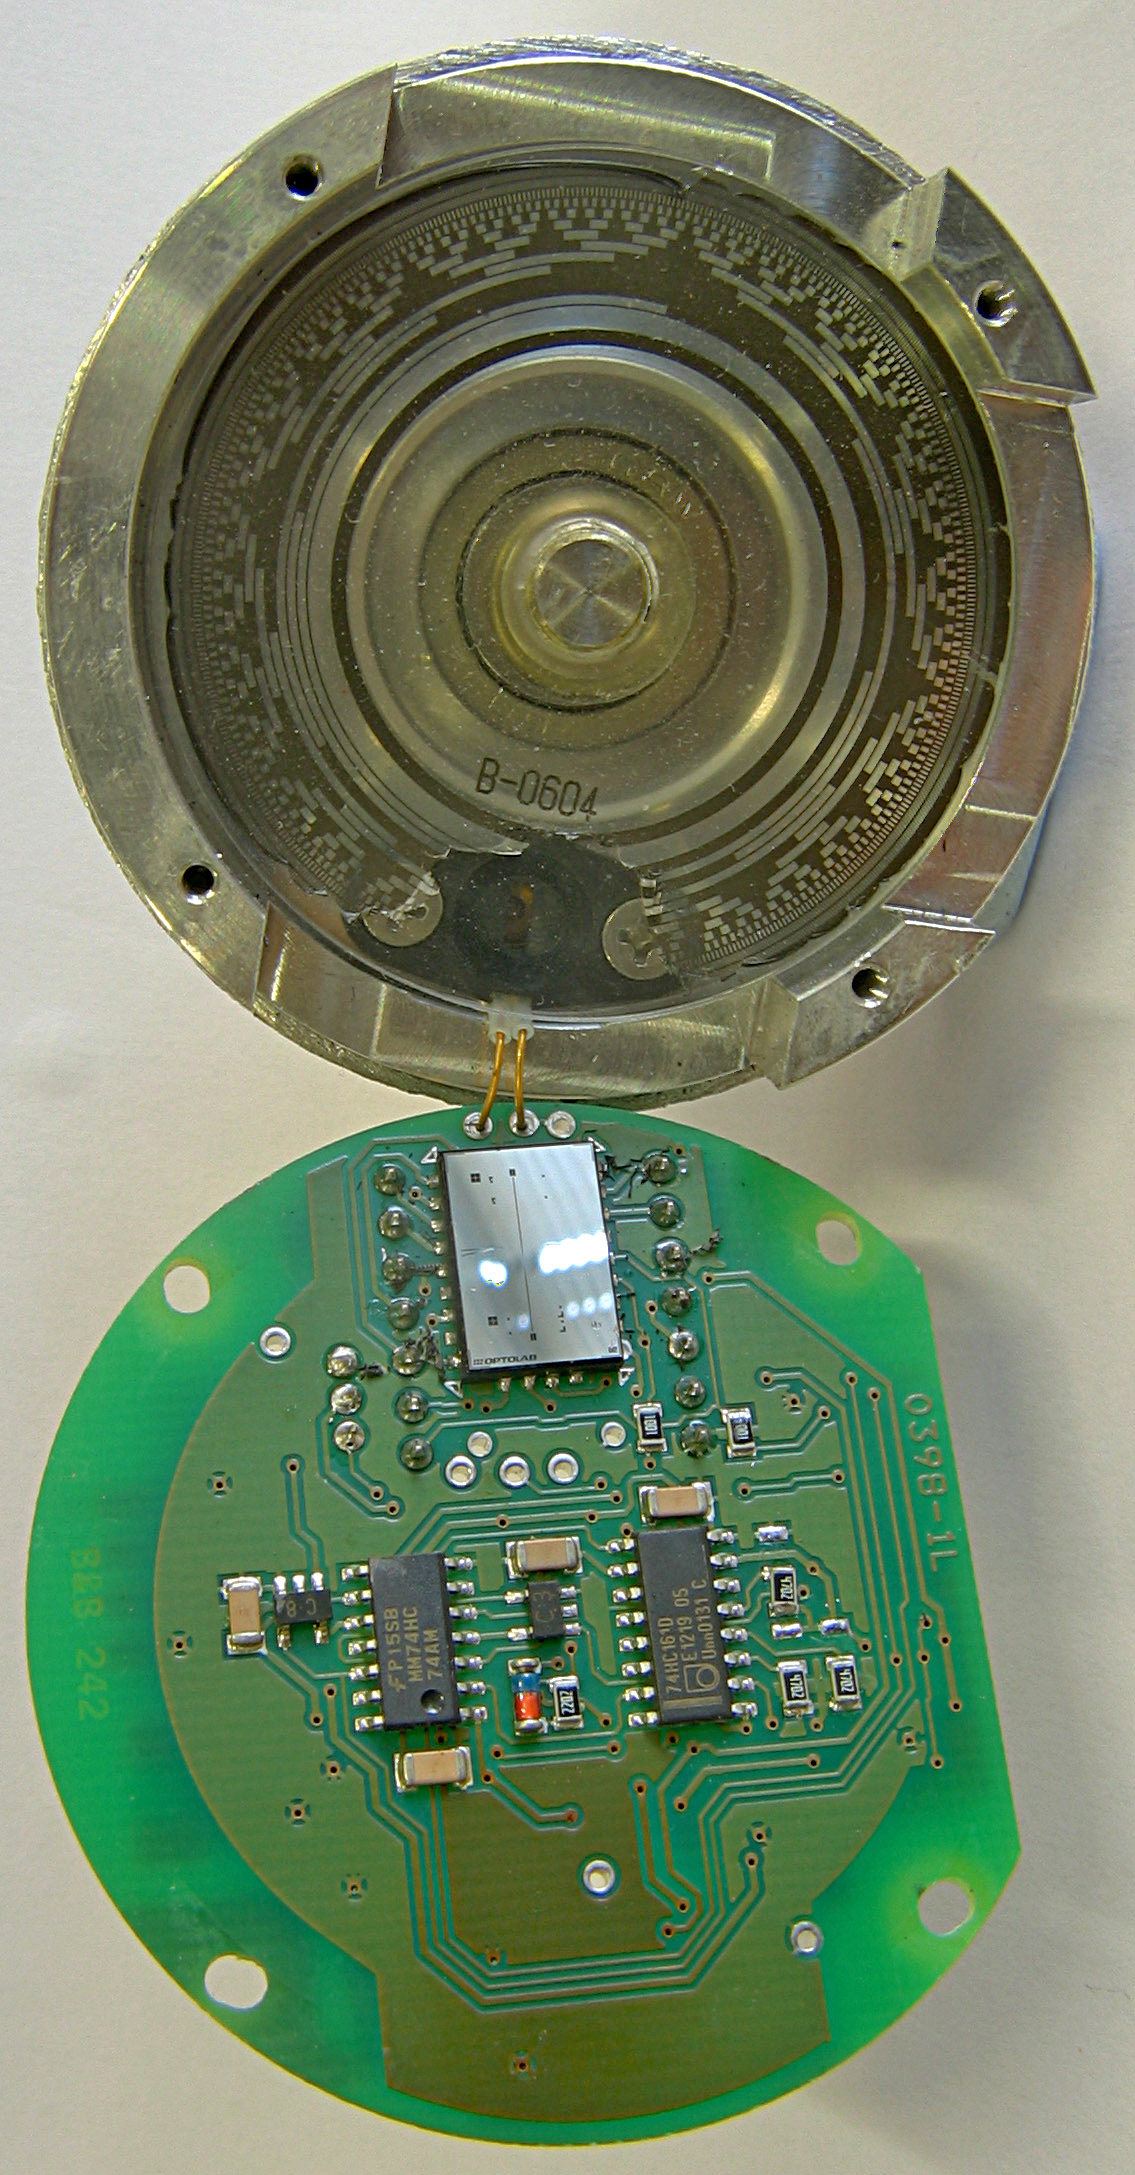
\includegraphics[height=3.2cm]{../../figures/d5_gray_encoder.jpg}\\
\credit{13-track Gray-code encoder, Mike1024, public domain, via Wikimedia Commons}
\column{.68\textwidth}
\begin{itemize}\small
\item \term{Absolute}: every angle has its own code (many tracks, Gray-coded) $\Rightarrow$ position known at switch-on, \hl{no homing}.
\item \term{Single-turn}: e.g.\ 17--23 bit per rev. \term{Multi-turn}: also counts whole revolutions (gears or a battery-backed counter).
\item Robots use multi-turn absolute encoders: after a power cut the arm knows its pose at once.
\end{itemize}
\small
\renewcommand{\arraystretch}{1.08}
\begin{tabularx}{\linewidth}{@{}l X@{}}
\toprule
\textbf{Protocol} & \textbf{Features}\\
\midrule
SSI & simple, one direction\\
BiSS-C, EnDat 2.2 & two-way, CRC check, diagnostics\\
\bottomrule
\end{tabularx}
\end{columns}
\end{frame}

% ---------------------------------------------------------------------
\begin{frame}{Resolver: a rotating transformer}
\begin{columns}[T]
\column{.55\textwidth}
\centering
\begin{tikzpicture}
\begin{groupplot}[group style={group size=1 by 3,vertical sep=1.5mm,xticklabels at=edge bottom},
  mkplot,width=\linewidth,xmin=0,xmax=10,ymin=-1.1,ymax=1.1,ytick=\empty]
\nextgroupplot[height=2.2cm,ylabel={$u_\text{ex}$}]
\addplot[mkMid,thin,domain=0:10,samples=401] {sin(720*x)};
\nextgroupplot[height=2.2cm,ylabel={$u_\text{sin}$}]
\addplot[mkBlue,thin,domain=0:10,samples=401] {sin(720*x)*sin(36*x)};
\addplot[mkOrange,thick,dashed,domain=0:10,samples=60] {sin(36*x)};
\nextgroupplot[height=2.2cm,ylabel={$u_\text{cos}$},xlabel={time [ms]}]
\addplot[mkBlue,thin,domain=0:10,samples=401] {sin(720*x)*cos(36*x)};
\addplot[mkOrange,thick,dashed,domain=0:10,samples=60] {cos(36*x)};
\end{groupplot}
\end{tikzpicture}
{\scriptsize\color{mkGray} Illustration: carrier \SI{2}{kHz}, rotor turning slowly.}
\column{.43\textwidth}
\begin{itemize}\small
\item Rotor coil fed with a sine \term{carrier} $u_\text{ex}$.
\item Two stator coils at $90^\circ$ pick up $\sin\theta$ and $\cos\theta$ times the carrier.
\item The angle is in the \hl{envelopes} (dashed): $\theta=\operatorname{atan2}(\sin,\cos)$.
\item No electronics in the motor: robust to heat, shock, vibration.
\end{itemize}
\gofurther{a \term{resolver-to-digital converter} (RDC) demodulates the signals and uses a small tracking loop to output angle and speed.}
\end{columns}
\end{frame}

% ---------------------------------------------------------------------
\begin{frame}{Speed from an encoder and the low-speed problem}
\begin{columns}[T]
\column{.5\textwidth}
\centering
\begin{tikzpicture}[xscale=.55,yscale=.55,font=\scriptsize]
  \foreach \x in {0.7,2.3,3.9,5.5,7.1,8.7,10.3}{ \draw[mkBlue,thick] (\x,0) -- (\x,1) -- (\x+.8,1) -- (\x+.8,0);}
  \draw[mkBlue,thick] (0,0) -- (11.5,0);
  \node[left] at (0,.5) {pulses};
  \foreach \x in {1.5,9.5}{ \draw[mkOrange,thick,dashed] (\x,-1.4) -- (\x,1.6);}
  \draw[{Latex}-{Latex},mkOrange] (1.5,1.9) -- (9.5,1.9) node[midway,above]{M: count pulses in $T_s$};
  \draw[{Latex}-{Latex},mkMid] (2.3,-1.0) -- (3.9,-1.0) node[midway,below]{T: time one pulse};
\end{tikzpicture}

\vspace{2mm}
\begin{itemize}\small
\item \term{M-method}: count pulses in a fixed time $T_s$: good at high speed.
\item \term{T-method}: time between two pulses: good at low speed.
\item Modern drives combine both.
\end{itemize}
\column{.47\textwidth}
\begin{keybox}[Worked example: M-method]
\small
1.\ $4N=10\,000$ counts/rev, $T_s=\SI{125}{\micro s}$\\[1mm]
2.\ One count per sample $=\dfrac{1}{10\,000\cdot125\cdot10^{-6}}=\SI{0.8}{rev/s}$\\[1mm]
3.\ $=\SI{48}{rpm}$: the smallest speed step\\[1mm]
4.\ At \SI{60}{rpm} the reading jumps between 48 and \SI{96}{rpm}!
\end{keybox}
\begin{notebox}
\small Remedies: more counts/rev, longer windows, filtering (W2D5, 6.6).
\end{notebox}
\end{columns}
\end{frame}

% ---------------------------------------------------------------------
\begin{frame}{Accelerometers: a mass on a spring}
\begin{columns}[T]
\column{.5\textwidth}
\centering
\begin{tikzpicture}[font=\scriptsize]
  \draw[thick,mkNavy] (0,0) rectangle (4,2);
  \draw[decorate,decoration={zigzag,segment length=2mm,amplitude=1.5mm},thick,mkMid] (0,1) -- (1.4,1);
  \draw[decorate,decoration={zigzag,segment length=2mm,amplitude=1.5mm},thick,mkMid] (2.4,1) -- (4,1);
  \draw[thick,mkNavy,fill=mkOrange] (1.4,.6) rectangle (2.4,1.4); \node[white] at (1.9,1) {$m$};
  \draw[mkGray,dashed] (1.6,.3) -- (1.6,1.7); \draw[{Latex}-{Latex},mkRed] (1.6,1.6) -- (1.9,1.6) node[right,font=\tiny]{$x$};
  \draw[sig] (1.2,-.4) -- (2.8,-.4) node[right]{case accelerates $a$};
  \node[mkGray] at (.7,.4) {$k$}; \node[mkGray] at (3.2,.4) {$k$};
  \draw[mkSky,thick] (2.45,.5) -- (2.45,1.5); \draw[mkSky,thick] (2.6,.5) -- (2.6,1.5); \node[mkSky,above,font=\tiny] at (2.55,1.5) {capacitor};
\end{tikzpicture}

\vspace{1mm}
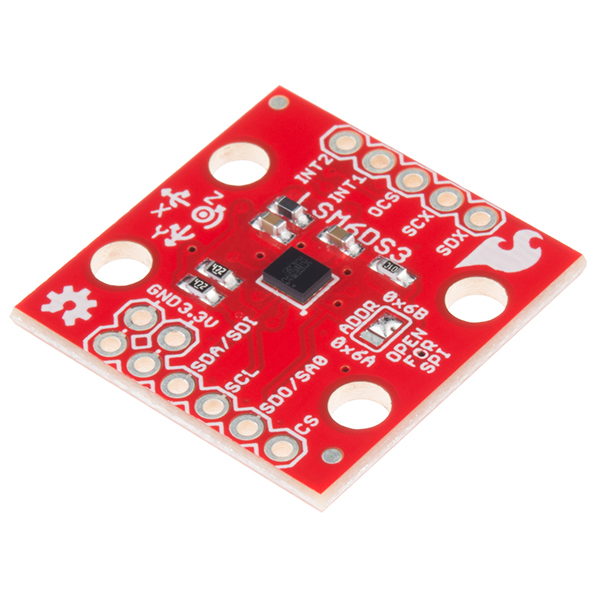
\includegraphics[height=1.9cm]{../../figures/r24_imu.jpg}\\
\credit{6-DoF IMU breakout (LSM6DS3), SparkFun, CC BY 2.0, via Wikimedia Commons}
\column{.48\textwidth}
\begin{eqbox}
\vspace{-2mm}
\[ x=\frac{m}{k}\,a \]
\vspace{-4mm}
\end{eqbox}
{\footnotesize $x$ deflection [m], $m$ proof mass [kg], $k$ spring stiffness [N/m], $a$ acceleration [m/s$^2$].}
\begin{itemize}\small
\item Silicon (\term{MEMS}) chip: a tiny mass moves, a capacitor measures $x$.
\item At rest it measures \hl{gravity}: $a_x=g\sin\theta$ gives tilt.
\end{itemize}
\begin{keybox}[Worked example: tilt]
\small
1.\ At rest, $a_x=\SI{4.9}{m/s^2}$, $g=\SI{9.81}{m/s^2}$\\
2.\ $\sin\theta=4.9/9.81=0.5$ $\Rightarrow$ $\theta=30^\circ$
\end{keybox}
\end{columns}
\end{frame}

% ---------------------------------------------------------------------
\begin{frame}{Gyroscopes and the IMU: drift and fusion}
\begin{columns}[T]
\column{.5\textwidth}
\centering
\begin{tikzpicture}
\begin{axis}[mkplot,width=\linewidth,height=4.4cm,xmin=0,xmax=10,ymin=-2,ymax=8,
  xlabel={time [min]},ylabel={angle error [$^\circ$]},legend pos=north west]
\addplot[mkOrange,thick,domain=0:10] {0.6*x};
\addplot[mkBlue,thick,domain=0:10,samples=200] {0.6*sin(deg(7*x))*exp(-0.0*x)*0.5+0.1*sin(deg(19*x))};
\legend{gyro only (bias \SI{0.01}{\degree/s}), gyro $+$ accelerometer (fused)}
\end{axis}
\end{tikzpicture}
\column{.48\textwidth}
\begin{itemize}\small
\item A \term{gyroscope} measures \hl{angular rate} $\omega$ [$^\circ$/s] (MEMS: vibrating mass + Coriolis force).
\item Angle $=$ integral of rate: a small \term{bias} grows into a large angle error (\term{drift}).
\item \term{IMU} $=$ 3-axis accelerometer $+$ 3-axis gyro (sometimes magnetometer).
\end{itemize}
\begin{keybox}[Worked example: drift]
\small Bias \SI{0.01}{\degree/s} $\times$ \SI{600}{s} (10 min) $=6^\circ$ error.
\end{keybox}
\gofurther{a complementary or Kalman filter trusts the gyro for fast changes and the accelerometer for the long-term tilt (W2D5, 6.6).}
\end{columns}
\end{frame}

% ---------------------------------------------------------------------
\begin{frame}{Check your understanding: position and motion sensors}
\begin{keybox}[Check your understanding]
\large
\begin{enumerate}
\item A 1000-line incremental encoder is decoded $\times4$. How many counts per revolution, and how many degrees per count?
\item After a power failure, which encoder type needs a homing run: incremental or absolute? Why?
\item An accelerometer at rest reads $a_x=\SI{9.81}{m/s^2}$. How is it tilted?
\end{enumerate}
\end{keybox}
\end{frame}

% ---------------------------------------------------------------------
\begin{frame}{Summary and key terms: position and motion sensors}
\begin{columns}[T]
\column{.52\textwidth}
\begin{itemize}\small
\item Motor-side encoder in every joint; gear multiplies resolution.
\item Incremental A/B/Z: $4N$ counts/rev, homing needed.
\item Absolute (Gray code, multi-turn): pose known at power-up.
\item Resolver: robust analogue sensor; angle from atan2.
\item IMU: accelerometer (tilt) $+$ gyro (rate, drifts).
\end{itemize}
\column{.45\textwidth}
\begin{defbox}[Key terms]
\small
\term{quadrature} two signals $90^\circ$ apart\\
\term{homing} finding a known zero position\\
\term{Gray code} one bit changes per step\\
\term{resolver} rotary transformer sensor\\
\term{MEMS} micro-machined silicon sensor\\
\term{drift} slowly growing error from bias
\end{defbox}
{\scriptsize\color{mkGray} [Siciliano \& Khatib, 2016]; [Fraden, 2016].}
\end{columns}
\end{frame}

% =====================================================================
\section{6.3 Force/torque, tactile, proximity and range sensors}

\begin{frame}{A map of robot sensors by what they detect}
\centering
\begin{tikzpicture}[font=\scriptsize]
  \draw[sig] (0,0) -- (13.4,0);
  \node[mkGray,above left] at (13.4,0) {distance to object};
  \foreach \x/\t in {.8/touch,3.5/mm,6.3/cm,9.1/m,12/10 m}{\node[mkGray,below] at (\x,0) {\t}; \draw[mkGray] (\x,0) -- (\x,.1);}
  \foreach \a/\b/\y/\t/\c in {0.2/1.6/.5/{force/torque, tactile}/mkOrange, 2.4/5.2/1.3/{inductive, capacitive}/mkBlue,
     4.4/10.6/.5/{photoelectric}/mkBlue, 5.6/10.2/2.1/{ultrasonic}/mkMid, 7.6/13.0/1.3/{LiDAR, laser scanner}/mkSky}{
    \draw[\c,line width=4pt] (\a,\y) -- (\b,\y);
    \node[above,font=\scriptsize,text=mkNavy] at ({(\a+\b)/2},\y+.05) {\t};}
\end{tikzpicture}

\vspace{4mm}
\begin{columns}[T]
\column{.5\textwidth}
\begin{itemize}\small
\item \term{Contact} sensors: force/torque, tactile skins, limit switches.
\item \term{Proximity} sensors: detect presence (yes/no) at short range.
\end{itemize}
\column{.47\textwidth}
\begin{itemize}\small
\item \term{Range} sensors: measure a distance (ultrasonic, LiDAR).
\item Many give a simple \hl{switching output} to a PLC input.
\end{itemize}
\end{columns}
\end{frame}

% ---------------------------------------------------------------------
\begin{frame}{Strain gauges and the Wheatstone bridge}
\begin{columns}[T]
\column{.36\textwidth}
\centering
\begin{circuitikz}[scale=.5,transform shape,font=\scriptsize]
  \draw (0,0) to[R,l=$R_1$] (2,2) to[R,l=$R_2$] (4,0);
  \draw (0,0) to[R,l_=$R_4$] (2,-2) to[R,l_=$R_3$] (4,0);
  \draw (0,0) -- (0,-2.8) to[V,l_=$U_\text{ex}$] (4,-2.8) -- (4,0);
  \draw (2,2) to[short,*-o] (2,2.5) node[above]{$u_+$};
  \draw (2,-2) to[short,*-o] (2,-1.5) node[right]{$u_-$};
\end{circuitikz}

\vspace{1mm}
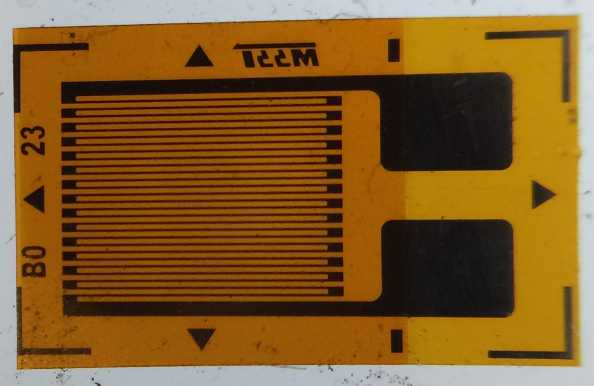
\includegraphics[height=1.7cm]{../../figures/d5_strain_gauge.jpg}\\
\credit{Foil strain gauge, Pleriche, CC BY-SA 4.0, via Wikimedia Commons}
\column{.62\textwidth}
\begin{itemize}\small
\item A \term{strain gauge} is a thin foil resistor glued on metal: stretch it and $R$ rises.
\item Changes are tiny, so we use a \term{Wheatstone bridge} (left) to measure them.
\end{itemize}
\begin{eqbox}
\vspace{-2mm}
\[
\frac{\Delta R}{R}=k_\text{GF}\,\varepsilon\qquad (k_\text{GF}\approx 2,\ \varepsilon=\text{strain}=\Delta L/L)
\]
\vspace{-4mm}
\end{eqbox}
\begin{keybox}[Worked example: full bridge]
\small
1.\ $\varepsilon=10^{-3}$, $U_\text{ex}=\SI{5}{V}$, 4 active gauges\\
2.\ $u_\text{out}\approx k_\text{GF}\,\varepsilon\,U_\text{ex}=2\cdot10^{-3}\cdot\SI{5}{V}=\SI{10}{mV}$\\
3.\ Millivolts $\Rightarrow$ needs a low-noise amplifier
\end{keybox}
{\small A \term{load cell} is a metal body with a bridge of gauges, rated in mV/V.}
\end{columns}
\end{frame}

% ---------------------------------------------------------------------
\begin{frame}{Six-axis force/torque sensor at the robot wrist}
\begin{columns}[T]
\column{.46\textwidth}
\centering
\begin{tikzpicture}[font=\scriptsize,x={(1cm,0)},y={(0,1cm)},z={(-.45cm,-.3cm)}]
  \draw[mkBlue,line width=5pt] (-1.8,1.6,0) -- (0,.55,0);
  \draw[thick,mkNavy,fill=mkSky!40] (-.9,.25) rectangle (.9,.55);
  \draw[thick,mkNavy,fill=mkCream] (-.9,0) rectangle (.9,.25);
  \node[right] at (.95,.27) {F/T sensor};
  \draw[thick,mkNavy,fill=mkPale] (-.3,0) rectangle (.3,-.9); \node at (0,-.45) {tool};
  \draw[-{Latex},thick,mkOrange] (0,-.95,0) -- (0,-1.9,0) node[below]{$F_z$};
  \draw[-{Latex},thick,mkOrange] (0,-.95,0) -- (1.2,-.95,0) node[right]{$F_x$};
  \draw[-{Latex},thick,mkOrange] (0,-.95,0) -- (0,-.95,1.6) node[left]{$F_y$};
  \draw[-{Latex},thick,mkMid] (1.5,-.2) arc (-60:240:.25 and .12); \node[mkMid] at (2.0,-.15) {$T_x,T_y,T_z$};
  \draw[{Latex}-{Latex},mkGray] (.3,-.6) -- (1.3,-.6) node[midway,above,font=\tiny]{$r$};
  \fill[mkRed] (1.3,-.6) circle (.06);
\end{tikzpicture}

\vspace{2mm}
\begin{itemize}\small
\item Strain gauges on a stiff metal cross measure \hl{3 forces + 3 torques}.
\item Uses: force-controlled grinding, insertion, collision detection, hand guiding.
\end{itemize}
\column{.52\textwidth}
\begin{defbox}[Refresher: torque]
\small Torque $=$ force $\times$ lever arm: $T=F\,r$ [N\,m].
\end{defbox}
\begin{keybox}[Worked example: subtract the tool]
\small
1.\ Gripper mass \SI{2}{kg}, centre of mass $r=\SI{0.1}{m}$ sideways\\
2.\ Weight $F_z=2\cdot9.81\approx\SI{19.6}{N}$\\
3.\ Torque $T=19.6\cdot0.1\approx\SI{1.96}{N\,m}$\\
4.\ The controller subtracts these (\term{gravity compensation}) so only \emph{contact} forces remain.
\end{keybox}
\begin{notebox}
\small The tool's weight changes direction as the wrist turns, so the compensation must use the current orientation.
\end{notebox}
\end{columns}
\end{frame}

% ---------------------------------------------------------------------
\begin{frame}{Tactile sensors: a skin for the gripper}
\begin{columns}[T]
\column{.45\textwidth}
\centering
\begin{tikzpicture}[scale=.36]
  \foreach \i in {0,...,9}{\foreach \j in {0,...,9}{
    \pgfmathsetmacro{\v}{100*exp(-((\i-4.5)^2+(\j-5)^2)/6)+60*exp(-((\i-7)^2+(\j-2)^2)/2)}
    \pgfmathtruncatemacro{\vv}{min(100,\v)}
    \fill[mkOrange!\vv!mkPale] (\i,\j) rectangle ++(.92,.92);}}
  \node[font=\scriptsize,below] at (5,-.2) {$10\times10$ taxel pressure map};
\end{tikzpicture}
\column{.53\textwidth}
\begin{itemize}\small
\item A \term{tactile sensor} is an array of small pressure cells (\term{taxels}), like the nerve endings in a fingertip.
\item Principles: resistive (pressure lowers $R$), capacitive (gap shrinks, $C$ rises), piezoelectric (dynamic, slip).
\item Gives \hl{where} and \hl{how hard} the object touches: detects slip, centres a grasp.
\end{itemize}
\begin{eqbox}
\vspace{-2mm}
\[ C=\varepsilon\,\frac{A}{d}\quad\Rightarrow\quad d\downarrow\ \ C\uparrow \]
\vspace{-4mm}
\end{eqbox}
{\footnotesize $C$ capacitance [F], $A$ plate area [m$^2$], $d$ gap [m], $\varepsilon$ permittivity [F/m].}
\end{columns}
\end{frame}

% ---------------------------------------------------------------------
\begin{frame}{Inductive and capacitive proximity sensors}
\begin{columns}[T]
\column{.45\textwidth}
\centering
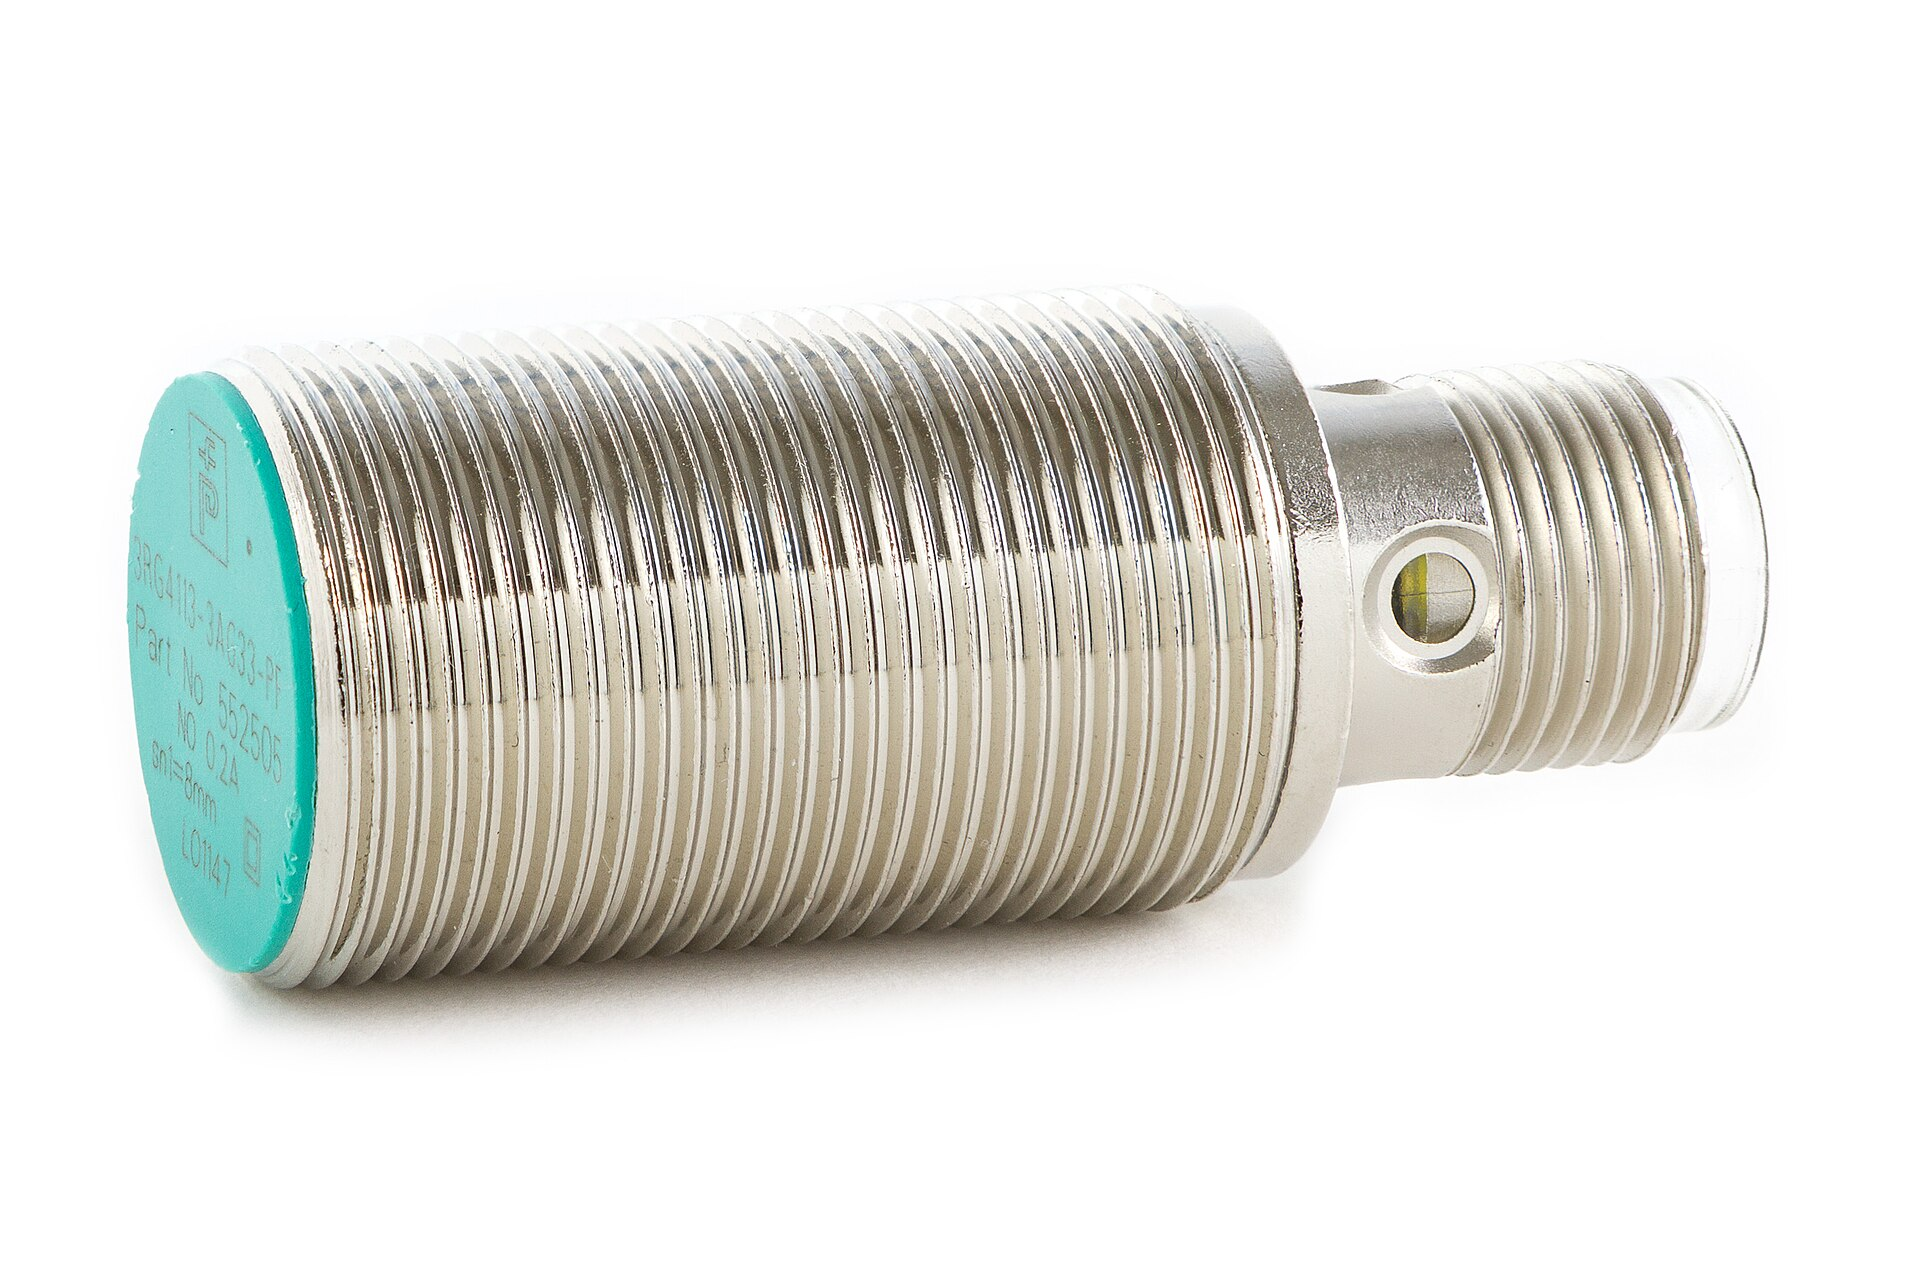
\includegraphics[width=.8\linewidth,height=2.3cm,keepaspectratio]{../../figures/r24_inductive.jpg}\\
\credit{Inductive proximity switch, Lucasbosch, CC BY-SA 3.0, via Wikimedia Commons}

\vspace{1mm}
\begin{tikzpicture}[font=\scriptsize]
  \draw[thick,mkNavy,fill=mkPale] (0,0) rectangle (2.2,.8); \node at (1.1,.4) {coil + oscillator};
  \foreach \r in {.3,.55,.8}{\draw[mkSky,thick] (2.2,.4) ++(-90:\r) arc (-90:90:\r);}
  \draw[fill=mkGray] (3.3,-.1) rectangle (3.6,.9); \node[right,align=left] at (3.6,.4) {metal\\target};
  \draw[{Latex}-{Latex},mkOrange] (2.2,-.3) -- (3.3,-.3) node[midway,below]{$s_n$};
\end{tikzpicture}
\column{.53\textwidth}
\begin{itemize}\small
\item \term{Inductive}: an AC magnetic field; nearby \hl{metal} absorbs energy (eddy currents) $\Rightarrow$ output switches.
\item \term{Capacitive}: an electric field; any material (plastic, liquid, wood) changes the capacitance.
\item \term{Sensing distance} $s_n$: a few mm; shrinks for non-steel metals.
\end{itemize}
\small
\renewcommand{\arraystretch}{1.05}
\begin{tabular}{@{}l c@{}}
\toprule
\textbf{Target (inductive)} & \textbf{factor on $s_n$}\\
\midrule
mild steel & 1.0\\
stainless steel & $\approx0.7$\\
aluminium, copper & $\approx0.3$--$0.4$\\
\bottomrule
\end{tabular}
\end{columns}
\end{frame}

% ---------------------------------------------------------------------
\begin{frame}{Photoelectric sensors: three ways to use a light beam}
\centering
\begin{tikzpicture}[font=\scriptsize]
  \foreach \i/\t in {0/Through-beam,1/Retro-reflective,2/Diffuse}{
    \node[font=\scriptsize\bfseries,text=mkBlue] at (\i*4.6+1.7,2.0) {\t};}
  % through beam
  \draw[thick,fill=mkPale] (0,.4) rectangle (.5,1.2); \node[font=\tiny] at (.25,.2) {emitter};
  \draw[thick,fill=mkPale] (3,.4) rectangle (3.5,1.2); \node[font=\tiny] at (3.25,.2) {receiver};
  \draw[mkOrange,thick,-{Latex}] (.5,.8) -- (3,.8);
  \draw[fill=mkGray] (1.5,.5) rectangle (1.9,1.1);
  % retro
  \draw[thick,fill=mkPale] (4.6,.4) rectangle (5.1,1.2); \node[font=\tiny] at (4.85,.2) {sensor};
  \draw[thick,fill=mkSky] (7.6,.4) rectangle (7.8,1.2); \node[font=\tiny] at (7.7,.2) {reflector};
  \draw[mkOrange,thick,-{Latex}] (5.1,.95) -- (7.6,.95); \draw[mkOrange,thick,-{Latex}] (7.6,.65) -- (5.1,.65);
  % diffuse
  \draw[thick,fill=mkPale] (9.2,.4) rectangle (9.7,1.2); \node[font=\tiny] at (9.45,.2) {sensor};
  \draw[fill=mkGray] (11.4,.4) rectangle (11.8,1.2); \node[font=\tiny] at (11.6,.2) {object};
  \draw[mkOrange,thick,-{Latex}] (9.7,.95) -- (11.4,.95); \draw[mkOrange,thick,dashed,-{Latex}] (11.4,.65) -- (9.7,.65);
\end{tikzpicture}

\vspace{3mm}
\small
\renewcommand{\arraystretch}{1.12}
\begin{tabularx}{\linewidth}{@{}l X X X@{}}
\toprule
 & \textbf{Through-beam} & \textbf{Retro-reflective} & \textbf{Diffuse}\\
\midrule
Detects when & beam is \hl{blocked} & beam is \hl{blocked} & light \hl{returns} from object\\
Range & longest (tens of m) & medium (several m) & short (cm to $\sim$\SI{1}{m})\\
Wiring & two units & one unit $+$ reflector & one unit\\
Weak spot & alignment & shiny objects & dark or far objects\\
\bottomrule
\end{tabularx}
\end{frame}

% ---------------------------------------------------------------------
\begin{frame}{Ultrasonic range sensors: listening for an echo}
\begin{columns}[T]
\column{.5\textwidth}
\centering
\begin{tikzpicture}[font=\scriptsize]
  \draw[thick,fill=mkPale] (0,0) rectangle (.7,1.2); \node[rotate=90] at (.35,.6) {\tiny transducer};
  \foreach \r in {.4,.8,1.2,1.6}{\draw[mkSky,thick] (.7,.6) ++(-30:\r) arc (-30:30:\r);}
  \draw[fill=mkGray] (3.6,-.1) rectangle (3.9,1.3); \node[right] at (3.9,.6) {object};
  \foreach \r in {.5,1.0}{\draw[mkOrange,thick] (3.6,.6) ++(150:\r) arc (150:210:\r);}
  \draw[{Latex}-{Latex},mkNavy] (.7,-.35) -- (3.6,-.35) node[midway,below]{$d$};
\end{tikzpicture}

\vspace{2mm}
\begin{tikzpicture}
\begin{axis}[mkplot,width=\linewidth,height=2.8cm,xmin=0,xmax=7,ymin=-1.2,ymax=1.2,ytick=\empty,
  xlabel={time [ms]}]
\addplot[mkBlue,thin,domain=0:.4,samples=60] {sin(deg(2*pi*10*x))};
\addplot[mkOrange,thin,domain=5.83:6.23,samples=60] {0.4*sin(deg(2*pi*10*x))};
\draw[{Latex}-{Latex},mkNavy] (axis cs:.2,-1.0) -- (axis cs:5.9,-1.0) node[midway,above,font=\tiny]{$t=\SI{5.83}{ms}$};
\end{axis}
\end{tikzpicture}
\column{.48\textwidth}
\begin{eqbox}
\vspace{-2mm}
\[ d=\frac{c\,t}{2} \]
\vspace{-4mm}
\end{eqbox}
{\footnotesize $c$ speed of sound ($\approx\SI{343}{m/s}$ at \SI{20}{\celsius}), $t$ echo time; divide by 2 for the round trip.}
\begin{keybox}[Worked example]
\small
1.\ Echo after $t=\SI{5.83}{ms}$\\
2.\ $d=343\cdot0.00583/2\approx\SI{1.0}{m}$\\
3.\ At \SI{40}{\celsius}, $c\approx\SI{355}{m/s}$: same echo now means \SI{1.035}{m} (3.5\,\% error if uncorrected).
\end{keybox}
\begin{itemize}\small
\item Works on glass and liquids; wide cone, slow, sensitive to temperature.
\end{itemize}
\end{columns}
\end{frame}

% ---------------------------------------------------------------------
\begin{frame}{LiDAR and laser scanners: range with light}
\begin{columns}[T]
\column{.36\textwidth}
\centering
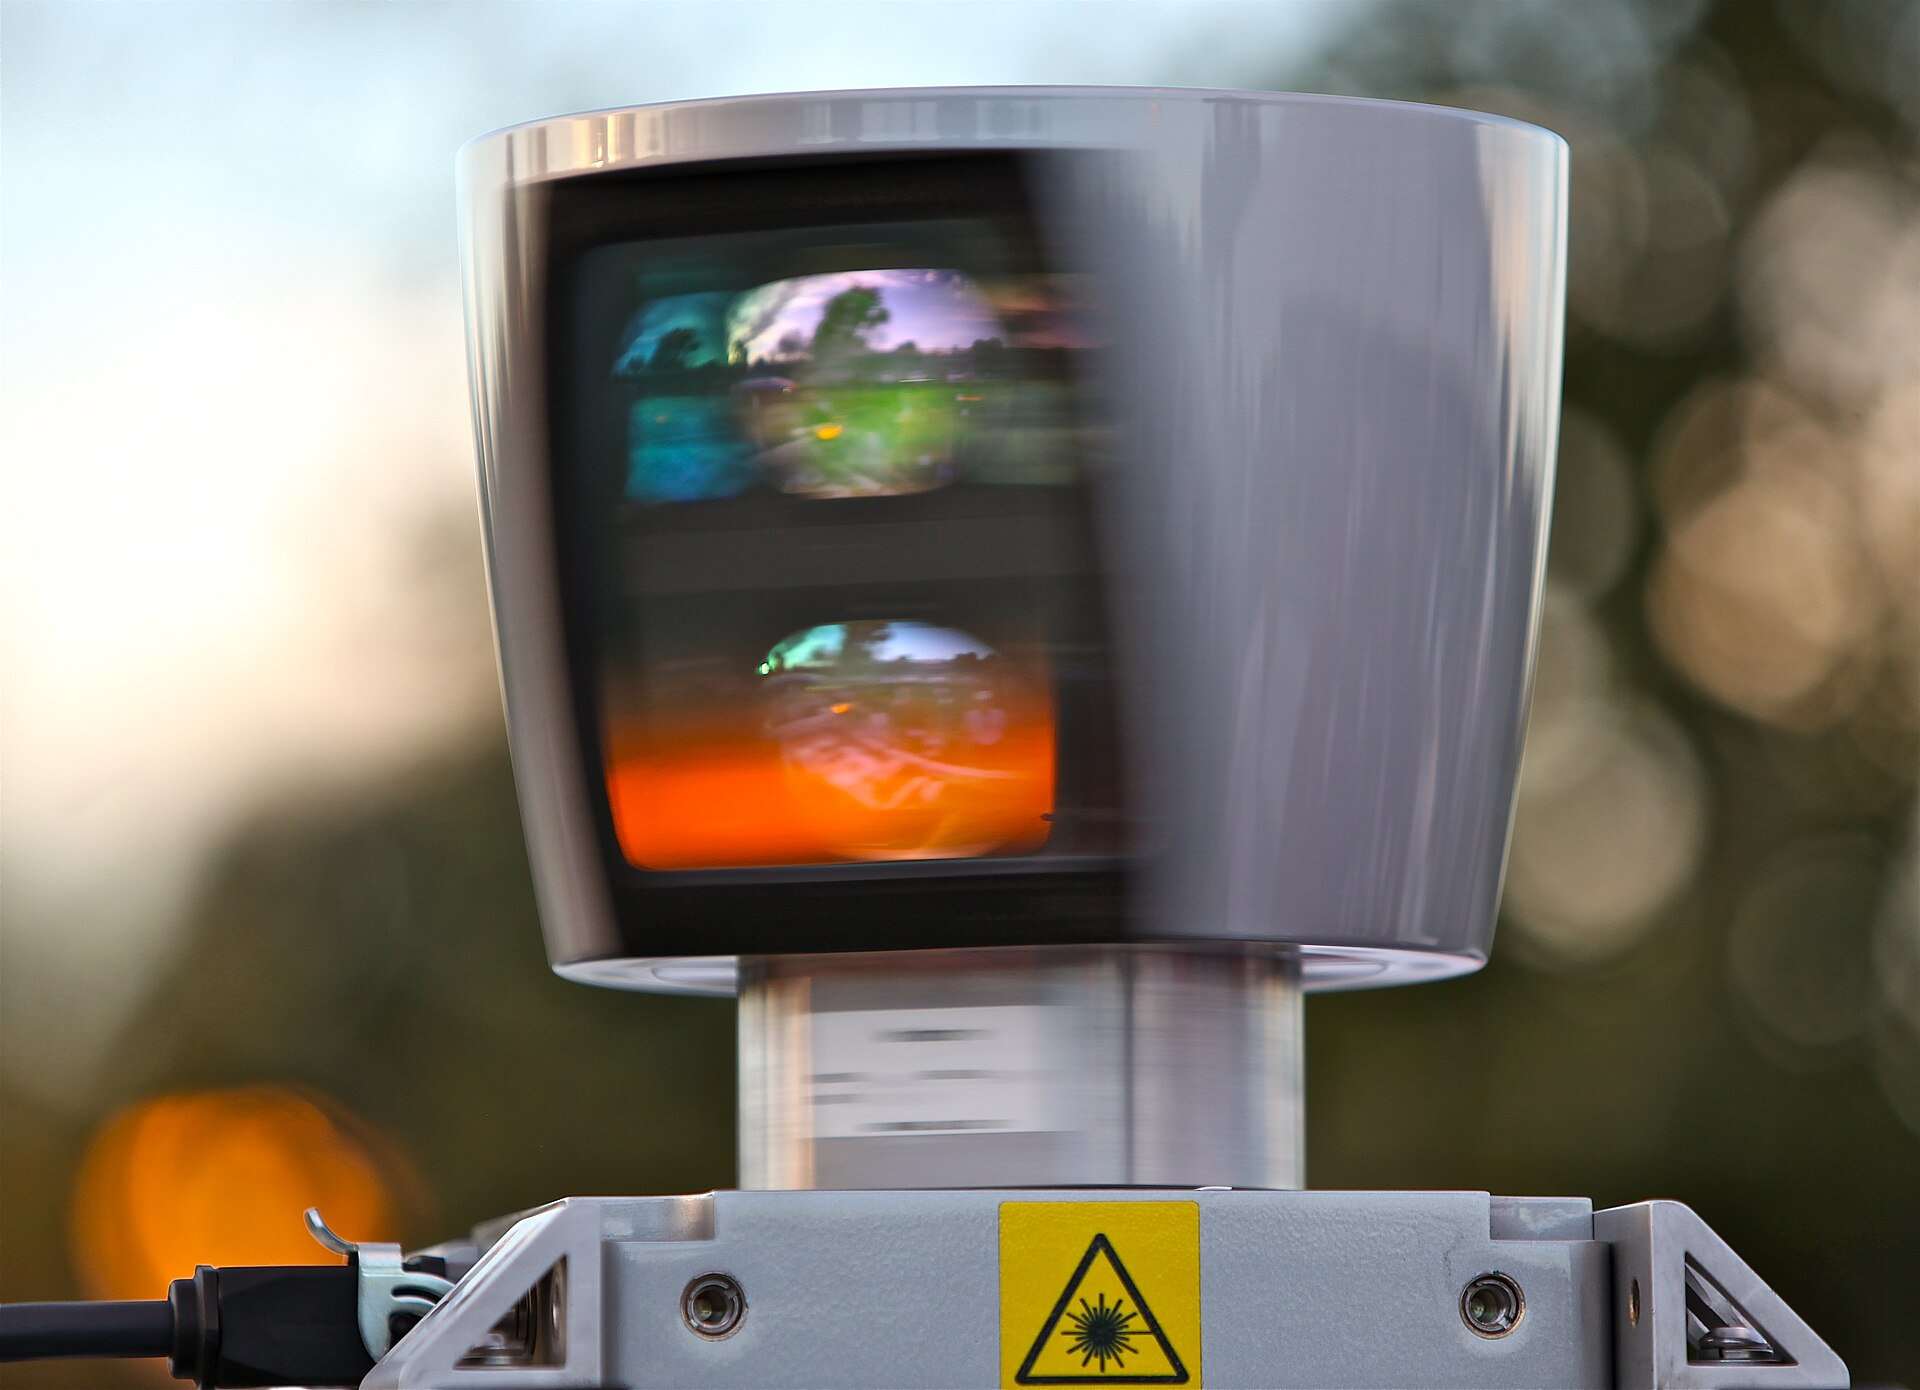
\includegraphics[width=\linewidth,height=3.0cm,keepaspectratio]{../../figures/r24_lidar.jpg}\\
\credit{Velodyne HDL-64E LiDAR, Steve Jurvetson, CC BY 2.0, via Wikimedia Commons}

\vspace{1mm}
\begin{tikzpicture}[font=\tiny,scale=.75]
  \fill[mkBlue] (0,0) circle (.12);
  \foreach \a in {0,6,...,180}{\pgfmathsetmacro{\r}{(\a<60)?2.2:((\a<120)?1.2/max(0.35,abs(sin(\a))):2.0)}
    \draw[mkSky,very thin] (0,0) -- (\a:\r); \fill[mkOrange] (\a:\r) circle (.04);}
  \node[below] at (0,-.1) {2-D scan};
\end{tikzpicture}
\column{.62\textwidth}
\begin{itemize}\small
\item \term{LiDAR} (light detection and ranging): a laser pulse, the same $d=c\,t/2$, but $c=\SI{3e8}{m/s}$.
\item A rotating mirror sweeps the beam $\Rightarrow$ a \term{point cloud} of distances.
\item 2-D \term{safety laser scanners} guard robot cells (Session 5.7); 3-D LiDARs guide AMRs.
\end{itemize}
\begin{keybox}[Worked example: nanoseconds]
\small
1.\ Object at \SI{1}{m}: $t=2d/c=2/(3\cdot10^8)\approx\SI{6.7}{ns}$\\
2.\ To resolve \SI{1}{cm} we must time $\approx\SI{67}{ps}$\\
3.\ That is why LiDARs need very fast electronics, while ultrasound is easy to time.
\end{keybox}
\end{columns}
\end{frame}

% ---------------------------------------------------------------------
\begin{frame}{Choosing a sensor for the task}
\small
\renewcommand{\arraystretch}{1.2}
\begin{tabularx}{\linewidth}{@{}X l l@{}}
\toprule
\textbf{Task in a robot cell} & \textbf{Good choice} & \textbf{Why}\\
\midrule
Is the steel part in the fixture? & inductive proximity & robust, cheap, metal only\\
Is the plastic bottle on the conveyor? & photoelectric (diffuse / retro) & any material, fast\\
Fill level of a bin of granules & ultrasonic & works on many surfaces\\
Insert a peg with \SI{5}{N} contact force & 6-axis F/T at the wrist & measures contact forces\\
Is the gripped object slipping? & tactile array & local pressure map\\
Person approaching the cell & safety laser scanner / light curtain & certified (PL d/e)\\
AMR navigation in a warehouse & LiDAR & accurate map of the room\\
\bottomrule
\end{tabularx}

\vspace{3mm}
\begin{notebox}
\small Ask four questions: \hl{what} material, \hl{how far}, \hl{yes/no or a value}, and \hl{is it safety-related?} Safety functions need certified safety sensors, not standard ones.
\end{notebox}
\end{frame}

% ---------------------------------------------------------------------
\begin{frame}{Check your understanding: force, proximity and range}
\begin{keybox}[Check your understanding]
\large
\begin{enumerate}
\item An inductive sensor has $s_n=\SI{8}{mm}$ for steel. Roughly how close must an aluminium part be?
\item An ultrasonic echo returns after \SI{2.9}{ms}. How far is the object (use \SI{343}{m/s})?
\item Why must a wrist F/T sensor ``subtract the tool'' before it can detect a collision?
\end{enumerate}
\end{keybox}
\end{frame}

% ---------------------------------------------------------------------
\begin{frame}{Summary and key terms: force, proximity and range}
\begin{columns}[T]
\column{.52\textwidth}
\begin{itemize}\small
\item Strain gauges in a bridge $\rightarrow$ load cells and 6-axis F/T sensors.
\item Tactile arrays give a pressure map for grasping.
\item Inductive (metal), capacitive (any material), photoelectric (light beam).
\item Range by time of flight: $d=ct/2$ (sound or light).
\item Choose by material, distance, output type, safety.
\end{itemize}
\column{.45\textwidth}
\begin{defbox}[Key terms]
\small
\term{Wheatstone bridge} measures tiny $\Delta R$\\
\term{F/T sensor} 3 forces $+$ 3 torques\\
\term{taxel} one tactile pressure cell\\
\term{sensing distance} $s_n$ switching range\\
\term{time of flight} echo time to distance\\
\term{point cloud} set of measured 3-D points
\end{defbox}
{\scriptsize\color{mkGray} [Fraden, 2016]; [Siciliano \& Khatib, 2016]; IEC 60947-5-2.}
\end{columns}
\end{frame}

% =====================================================================
\section{Day summary and outlook}

\begin{frame}{Day summary}
\begin{columns}[T]
\column{.55\textwidth}
\centering
\begin{tikzpicture}[font=\scriptsize,node distance=3mm,
  bx/.style={draw=mkBlue,fill=mkPale,thick,rounded corners=2pt,text width=5.8cm,align=left,minimum height=7mm}]
  \node[bx] (a) {\textbf{5.6} Conveyors, AGV/AMR, FMS, cobots: move parts, share space};
  \node[bx,below=of a] (b) {\textbf{5.7} ISO 12100 loop, PL$_\text{r}$, $S=KT+C$, stop categories};
  \node[bx,below=of b] (c) {\textbf{6.1} Measurement chain; accuracy, precision, resolution; calibration; $\tau$};
  \node[bx,below=of c] (d) {\textbf{6.2} Encoders (incremental, absolute), resolver, IMU};
  \node[bx,below=of d] (e) {\textbf{6.3} F/T, tactile, inductive, capacitive, photoelectric, ultrasonic, LiDAR};
\end{tikzpicture}
\column{.42\textwidth}
\begin{keybox}[Today in one sentence]
\small A flexible, safe robot cell depends on sensors: they tell the robot where it is, where the parts are, and where the people are.
\end{keybox}
\begin{defbox}[Three numbers to remember]
\small
$v=\pi D n/i$ \quad conveyor speed\\[1mm]
$S=K\,T+C$ \quad safety distance\\[1mm]
$d=c\,t/2$ \quad time-of-flight range
\end{defbox}
\end{columns}
\end{frame}

% ---------------------------------------------------------------------
\begin{frame}{Preview of tomorrow (W2D5): sensing, signals and integration}
\begin{columns}[T]
\column{.5\textwidth}
\small
\renewcommand{\arraystretch}{1.15}
\begin{tabularx}{\linewidth}{@{}l X@{}}
\toprule
\textbf{Code} & \textbf{Session}\\
\midrule
6.4 & Machine vision in robotics\\
6.5 & Sampling and digitisation\\
6.6 & Signal processing and filters\\
6.7 & Communication and integration\\
6.8 & System-integration case study \& wrap-up\\
\bottomrule
\end{tabularx}
\column{.47\textwidth}
\begin{defbox}[Questions to think about]
\small
\checkitem\ How does a camera tell the robot where a part is?\\[1mm]
\checkitem\ How often must we sample an encoder or a force sensor?\\[1mm]
\checkitem\ How do 50 sensors and 6 drives share one network in time?
\end{defbox}
\end{columns}
\end{frame}

% ---------------------------------------------------------------------
\begin{frame}{Figure credits}
\scriptsize
All plots and diagrams not listed here are original drawings made for this course (TikZ / pgfplots / circuitikz).

\vspace{2mm}
\renewcommand{\arraystretch}{1.15}
\begin{tabularx}{\linewidth}{@{}l X l l@{}}
\toprule
\textbf{File} & \textbf{Wikimedia Commons title} & \textbf{Author} & \textbf{License}\\
\midrule
\texttt{r24\_agv.jpg} & AGV - Automated Guided Vehicle.jpg & Marta Veverica & CC BY-SA 4.0\\
\texttt{r24\_cobot.png} & UR16e robot arm.png & Auledas & CC BY-SA 4.0\\
\texttt{r24\_imu.jpg} & SparkFun 6DoF-Breakout Gyroscope+Accelerometer LSM6DS3 13339-01.jpg & SparkFun & CC BY 2.0\\
\texttt{r24\_inductive.jpg} & Pepperl+Fuchs inductive proximity switch 3RG4113-3AG33-PF.jpg & Lucasbosch & CC BY-SA 3.0\\
\texttt{r24\_lidar.jpg} & Velodyne High-Def LIDAR.jpg & Steve Jurvetson & CC BY 2.0\\
\texttt{d5\_encoder\_model.jpg} & Encoder.jpg & Rrudzik & CC BY-SA 4.0\\
\texttt{d5\_gray\_encoder.jpg} & Gray code rotary encoder 13-track opened.jpg & Mike1024 & Public domain\\
\texttt{d5\_strain\_gauge.jpg} & Unmounted strain gauge.jpg & Pleriche & CC BY-SA 4.0\\
\bottomrule
\end{tabularx}

\vspace{1mm}
All via Wikimedia Commons (commons.wikimedia.org); licences as stated.
\end{frame}

% ---------------------------------------------------------------------
\begin{frame}{References}
\scriptsize
\begin{itemize}
\item M.~P.~Groover, \emph{Automation, Production Systems, and Computer-Integrated Manufacturing}, 5th ed., Pearson, 2019.
\item B.~Siciliano, O.~Khatib (eds.), \emph{Springer Handbook of Robotics}, 2nd ed., Springer, 2016.
\item J.~J.~Craig, \emph{Introduction to Robotics: Mechanics and Control}, 4th ed., Pearson, 2017.
\item J.~Fraden, \emph{Handbook of Modern Sensors}, 5th ed., Springer, 2016.
\item J.~P.~Bentley, \emph{Principles of Measurement Systems}, 4th ed., Pearson, 2005.
\item ISO 12100 (risk assessment and risk reduction); ISO 13849-1 (safety-related parts of control systems); IEC 62061.
\item ISO 10218-1/-2 (industrial robots, robot systems and integration); ISO/TS 15066 (collaborative robots).
\item ISO 13855 (positioning of safeguards); IEC 61496 (electro-sensitive protective equipment); IEC 60204-1 (electrical equipment of machines).
\item ISO 9283 (robot performance criteria); IEC 60947-5-2 (proximity switches).
\end{itemize}
\end{frame}

\end{document}
